% Copyright (c) 2008-2009 solvethis
% Copyright (c) 2010-2016 Casper Ti. Vector
% Public domain.
%
% 使用前请先仔细阅读 pkuthss ` biblatex-caspervector 的文档,
% 特别是其中的 FAQ 部分和用红色强调的部分。
% 两者可在终端/命令提示符中用
%   texdoc pkuthss
%   texdoc biblatex-caspervector
% 调出。

% 采用了自定义的(包括大小写不同于原文件的)字体文件名,
% 并改动 ctex.cfg 等配置文件的用户请自行加入 nofonts 选项;
% 其它用户不用加入 nofonts 选项,加入之后反而会产生错误。
\documentclass[UTF8,openany]{pkuthss}

% 使用 biblatex 排版参考文献,并规定其格式(详见 biblatex-caspervector 的文档)。
% 这里按照英文文献在前,中文文献在后排序(“sorting = ecnty”);
% 若需按照中文文献在前,英文文献在后排序,请设置“sorting = centy”;
% 若需按照引用顺序排序,请设置“sorting = none”。
% 若需在排序中实现更复杂的需求,请参考 biblatex-caspervector 的文档。
\usepackage[backend = biber, style = caspervector, utf8, sorting = ecnty, giveninits = true, sortgiveninits = true]{biblatex}
\usepackage{graphicx}
\usepackage{fancyvrb}
\usepackage{hologo}
%\usepackage{epsfig}
% 按学校要求设定参考文献列表中的条目之内及之间的距离。
\setlength{\bibitemsep}{3bp}
% 对于 linespread 值的计算过程有兴趣的同学可以参考 pkuthss.cls。
\renewcommand*{\bibfont}{\zihao{5}\linespread{1.27}\selectfont}

% 设定文档的基本信息。
\pkuthssinfo{
	cthesisname = {本科生学位论文}, ethesisname = {Doctor Thesis},
	ctitle = {针对高速SSD的KV接口标准实现与测试}, etitle = {Implementation and benchmark of standard KV interface aimed at high speed SSD},
	cauthor = {王润辉},
	eauthor = {Runhui Wang},
	studentid = {1200018504},
	date = {2016年5月},
	school = {信息科学技术学院},
	cmajor = {计算机科学与技术}, emajor = {Computer science and technology},
	direction = {计算机体系与结构},
	cmentor = {孙广宇}, ementor = {Prof.\ Guangyu Sun},
	ckeywords = {KV存储,统一接口,YCSB}, ekeywords = {KV Store,Framework, YCSB}
}
% 载入参考文献数据库(注意不要省略“.bib”)。
\addbibresource{thesis.bib}

% 普通用户可删除此段,并相应地删除 chap/*.tex 中的
% “\pkuthssffaq % 中文测试文字。”一行。
\usepackage{color}
\def\pkuthssffaq{%
	\emph{\textcolor{red}{pkuthss 文档模版最常见问题:}}

	\texttt{\string\cite}、\texttt{\string\parencite} %
	和 \texttt{\string\supercite} 三个命令分别产生%
	未格式化的、带方括号的和上标且带方括号的引用标记:%
	\cite{test-en},\parencite{test-zh}、\supercite{test-en, test-zh}。

	若要避免章末空白页,请在调用 pkuthss 文档类时加入 \texttt{openany} 选项。

	如果编译时不出参考文献,
	请参考 \texttt{texdoc pkuthss}“问题及其解决”一章
	“其它可能存在的问题”一节中关于 biber 的说明。
}

\begin{document}
	% 以下为正文之前的部分,默认不进行章节编号。
	\frontmatter
	% 此后到下一 \pagestyle 命令之前不排版页眉或页脚。
	\pagestyle{empty}
	% 自动生成封面。
	\maketitle
	% 版权声明。封面要求单面打印,故需新开右页。
	\cleardoublepage
%	% Copyright (c) 2008-2009 solvethis
% Copyright (c) 2010-2016 Casper Ti. Vector
% All rights reserved.
%
% Redistribution and use in source and binary forms, with or without
% modification, are permitted provided that the following conditions are
% met:
%
% * Redistributions of source code must retain the above copyright notice,
%   this list of conditions and the following disclaimer.
% * Redistributions in binary form must reproduce the above copyright
%   notice, this list of conditions and the following disclaimer in the
%   documentation and/or other materials provided with the distribution.
% * Neither the name of Peking University nor the names of its contributors
%   may be used to endorse or promote products derived from this software
%   without specific prior written permission.
%
% THIS SOFTWARE IS PROVIDED BY THE COPYRIGHT HOLDERS AND CONTRIBUTORS "AS
% IS" AND ANY EXPRESS OR IMPLIED WARRANTIES, INCLUDING, BUT NOT LIMITED TO,
% THE IMPLIED WARRANTIES OF MERCHANTABILITY AND FITNESS FOR A PARTICULAR
% PURPOSE ARE DISCLAIMED. IN NO EVENT SHALL THE COPYRIGHT HOLDER OR
% CONTRIBUTORS BE LIABLE FOR ANY DIRECT, INDIRECT, INCIDENTAL, SPECIAL,
% EXEMPLARY, OR CONSEQUENTIAL DAMAGES (INCLUDING, BUT NOT LIMITED TO,
% PROCUREMENT OF SUBSTITUTE GOODS OR SERVICES; LOSS OF USE, DATA, OR
% PROFITS; OR BUSINESS INTERRUPTION) HOWEVER CAUSED AND ON ANY THEORY OF
% LIABILITY, WHETHER IN CONTRACT, STRICT LIABILITY, OR TORT (INCLUDING
% NEGLIGENCE OR OTHERWISE) ARISING IN ANY WAY OUT OF THE USE OF THIS
% SOFTWARE, EVEN IF ADVISED OF THE POSSIBILITY OF SUCH DAMAGE.

% 此处不用 \specialchap,因为学校要求目录不包括其自己及其之前的内容。
\chapter*{版权声明}
% 综合学校的书面要求及 Word 模版来看,版权声明页不需加页眉、页脚。
\thispagestyle{empty}

任何收存和保管本论文各种版本的单位和个人,
未经本论文作者同意,不得将本论文转借他人,
亦不得随意复制、抄录、拍照或以任何方式传播。
否则一旦引起有碍作者著作权之问题,将可能承担法律责任。

% 若需排版二维码,请将二维码图片重命名为“barcode”,
% 转为合适的图片格式,并放在当前目录下,然后去掉下面 3 行的注释。
%\vfill\noindent
%\includegraphics[height = 5em]{barcode}

% vim:ts=4:sw=4


	% 此后到下一 \pagestyle 命令之前正常排版页眉和页脚。
	\cleardoublepage
	\pagestyle{plain}
	% 重置页码计数器,用大写罗马数字排版此部分页码。
	\setcounter{page}{0}
	\pagenumbering{Roman}
	% 中英文摘要。
	% Copyright (c) 2014,2016 Casper Ti. Vector
% Public domain.

\begin{cabstract}
	随着存储技术的迅速发展,当今以KV存储系统为代表的NoSQL数据库出现了百花齐放的状况,在不同的应用领域有着许多针对硬盘或者SSD的开源KV存储项目,然而它们都有着各自定义的KV API接口,上层应用为了实现相同的语义需要针对不同的KV存储分别搭建不同的适配器。为了减少适配器的重复开发,可以提出一个通用的KV框架——KVF ,其定义的API的语义概括了通用的KV模型,使上层应用可以使用一个统一的API接口来访问下层的KV存储。因此,KVF简化了基于KV模型的应用的开发过程。

	为了验证KV Framework(KVF)底层的实用性,我将Fusion-io盘与KVF框架对接,并开发Benchmark框架下的测试工具并进行端到端功能/性能测试。

	YCSB是雅虎云服务测试的简称,是用来测试cloud serving/NoSQL/Key-Value Store的测试工具。由于云服务的流行,传统数据库不能满足可利用性、可扩展性等要求,因此功能简化、一致性简化的NoSQL数据库逐渐流行。然而NoSQL数据库种类繁多,针对不同目的数据库各有权衡(读写性能、延迟和持久性、同步和异步等等),用户和开发人员需要针对不同的应用场景选择合适的数据库。YCSB的目标是提供一个公平测试的平台,为这些数据库提供一个统一的测试方案,从而更公平地在不同的方面衡量不同的数据库性能,从而提供有价值的参考。

	通过将YCSB与KVF进行连接,我们可以验证KVF的性能,为将来KVF与各种NoSQL数据库的整合打好基础。

\end{cabstract}

\begin{eabstract}
	With the rapid development of storage technology, there exist a variety of NoSQL databases which is represented by KV storage system. There are many open-source KV storage projects for specific disks in different fields. However, their KV APIs are different from each other so upper lever applications have to implement different adapters for different KV storages. To avoid developing different adapters in the same application, we can design a general KV framework, whose API concludes general KV model. Therefore, upper level applications can call unified interface to access lower lever KV storage. In this case, KVF simplifies the process of developing applications which are based on KV model.
	
	To testify the utility of KV Framework, I will connect Fusion-disk with KVF and develop a benchmark tool to perform peer-to-peer tests of functionality and performance.
\end{eabstract}

% vim:ts=4:sw=4

	% 自动生成目录。
	\tableofcontents

	% 以下为正文部分,默认要进行章节编号。
	\mainmatter
	% 序言。
	% Copyright (c) 2014,2016 Casper Ti. Vector
% Public domain.

\specialchap{序言}
%\pkuthssffaq % 中文测试文字。
	在做这个项目的开发过程中遇到了一系列的问题,在探索这些问题的过程中,自己也从对很多知识的一知半解到熟练使用,比如git版本控制、服务器上的各种权限问题、开源项目的编译配置、makefile的编写以及c和java语言的编译链接问题等等。在学以致用的过程中,总是充满了未知的挑战,很多时候会在某个问题卡住很久,但是当解决了一个个棘手的问题之后,内心的喜悦会证明之前的付出都是值得的。做毕业设计是一个不断探索未知,不断挑战自己的过程,在这个过程中不仅我的研究能力得到了锻炼,而且处理问题的能力也得到了很大提升。

	本文将由两个部分构成:
	\begin{itemize}
	\item \textbf{KVF}:
		%其中根据学校的格式规范\mbox{\supercite{pku-thesisstyle}}%
		该部分描述了KVF的基本原理和设计思路
		主要包括KVF的数据模型、系统架构、应用场景
		此外也介绍了一些基本的API
		
	\item \textbf{Benchmark的实现}:
		该部分介绍如何实现Benchmark
		主要内容包括如何依托开源项目YCSB(Yahoo! Cloud Serving Benchmark)实现Benchmark以及一些基本的测试结果与分析

	\end{itemize}
% vim:ts=4:sw=4

	% 各章节。
	% Copyright (c) 2014,2016 Casper Ti. Vector
% Public domain.
\chapter{KV Framework设计}
% \pkuthssffaq % 中文测试文字。
% vim:ts=4:sw=4
\section{概览}\label{sec:req}
	这部分将介绍键值对框架(Key Value Framework)的概念、概述以及接口的定义。KVF定义了统一的数据模型、函数和参数。通过这样一个框架,不同的Key value storage可以注册和注销注册,像虚拟文件系统管理ext3、jfs一样。此外该框架提供了统一的API以便上层应用调用,从而避免了同一个应用为了在不同厂商的的KV store实现功能而开发多个适配器的情况。

\section{键值存储(Key Value Store)介绍}\label{sec:doc-dir}
	

		传统的存储系统是基于SCSI架构的,客户端使用逻辑块地址(Logical Block Address,LBA)进行读写数据。在块的基础上我们可以提供更多的服务,比如文件系统、数据库等等。作为替代品,键值存储(也称为目标存储系统)提供了键值对操作。上层应用通过指定键名来存储数据值,键的名字可以是一个字符串变量,数据值可以是一个数据缓冲变量,这样上层应用可以很容易地存储数据,不需要基于线性块空间的复杂的布局设计,只需要聚焦于键名策略的设计和如何存储键名(比如使用分布式哈希表存储)。基于键值存储我们可以很容易地构造文件、swift、hdfs、no-sql甚至是块服务,如图1所示。
	\begin{center}
		\includegraphics[width=13.9cm]{img/figure1.pdf}
	\end{center}
	\centerline {图1}
	%\includepdf{figure1.pdf}
	%\epsfig{figure=figure1,height=6.4cm}
	
		实际上512或者4096字节大小的块设备是一种简单的键值存储,它的键名是LBA(Logical Block Address),数据值是512或者4096个字节大小的数据,因为这种简单性,上层应用需要复杂的布局设计(比如RamCloud),而数据大小可变的键值存储更加灵活,所以上层应用可以很容易在上面存储数据,这是一种性能和可用性之间的权衡。根据冗余的多少,键值存储可以分为三类:
	\begin{itemize}
		\item \textbf{独立的KVS}:
		
			独立的KVS是指如下的应用场景:
			应用客户端直接从一个独立的设备读写数据,比如从一个单独的硬盘、闪存卡等等。相关的产品包括希捷的Kineitic以及闪迪的Fusionio等等

		\item \textbf{分布式KVS}:
		
			分布式KVS是指如下应用场景:
			数据储存在多个服务器节点之间存在冗余,通过某种方式相互通信从而将这些服务器节点的存储资源整合到一起,并应用客户端提供读写接口。相关产品包括Ceph、mongoDB等等。

		\item \textbf{多数据中心的KVS}:
		
			多数据中心的KVS应用于如下场景:
			数据在多重数据中心都有冗余,有复制备份和纠删码的特性,相关的产品包括Amazon S3、SWIFT等等。
	\end{itemize}

		这三种KVS是有关联的,但是可以相互独立,例如多数据中心的KVS可以是基于分布式KVS的,分布式KVS页可以是基于独立KVS的。
\section{Key Value Framework (KVF) 数据模型}\label{sec:KVF-model}
	通过Key Value Framework(KVF)不同的厂商可以通过注册自己的Key Value库(KV-LIB)来管理它的Key Value Storage(KVS)。 这些KV-LIB应该遵循KVF数据模型,KVS提供pool,pool提供对象。pool支持嵌套设计,这意味着一个pool可以在另一个pool的上面,如图2所示。
	\begin{center}
		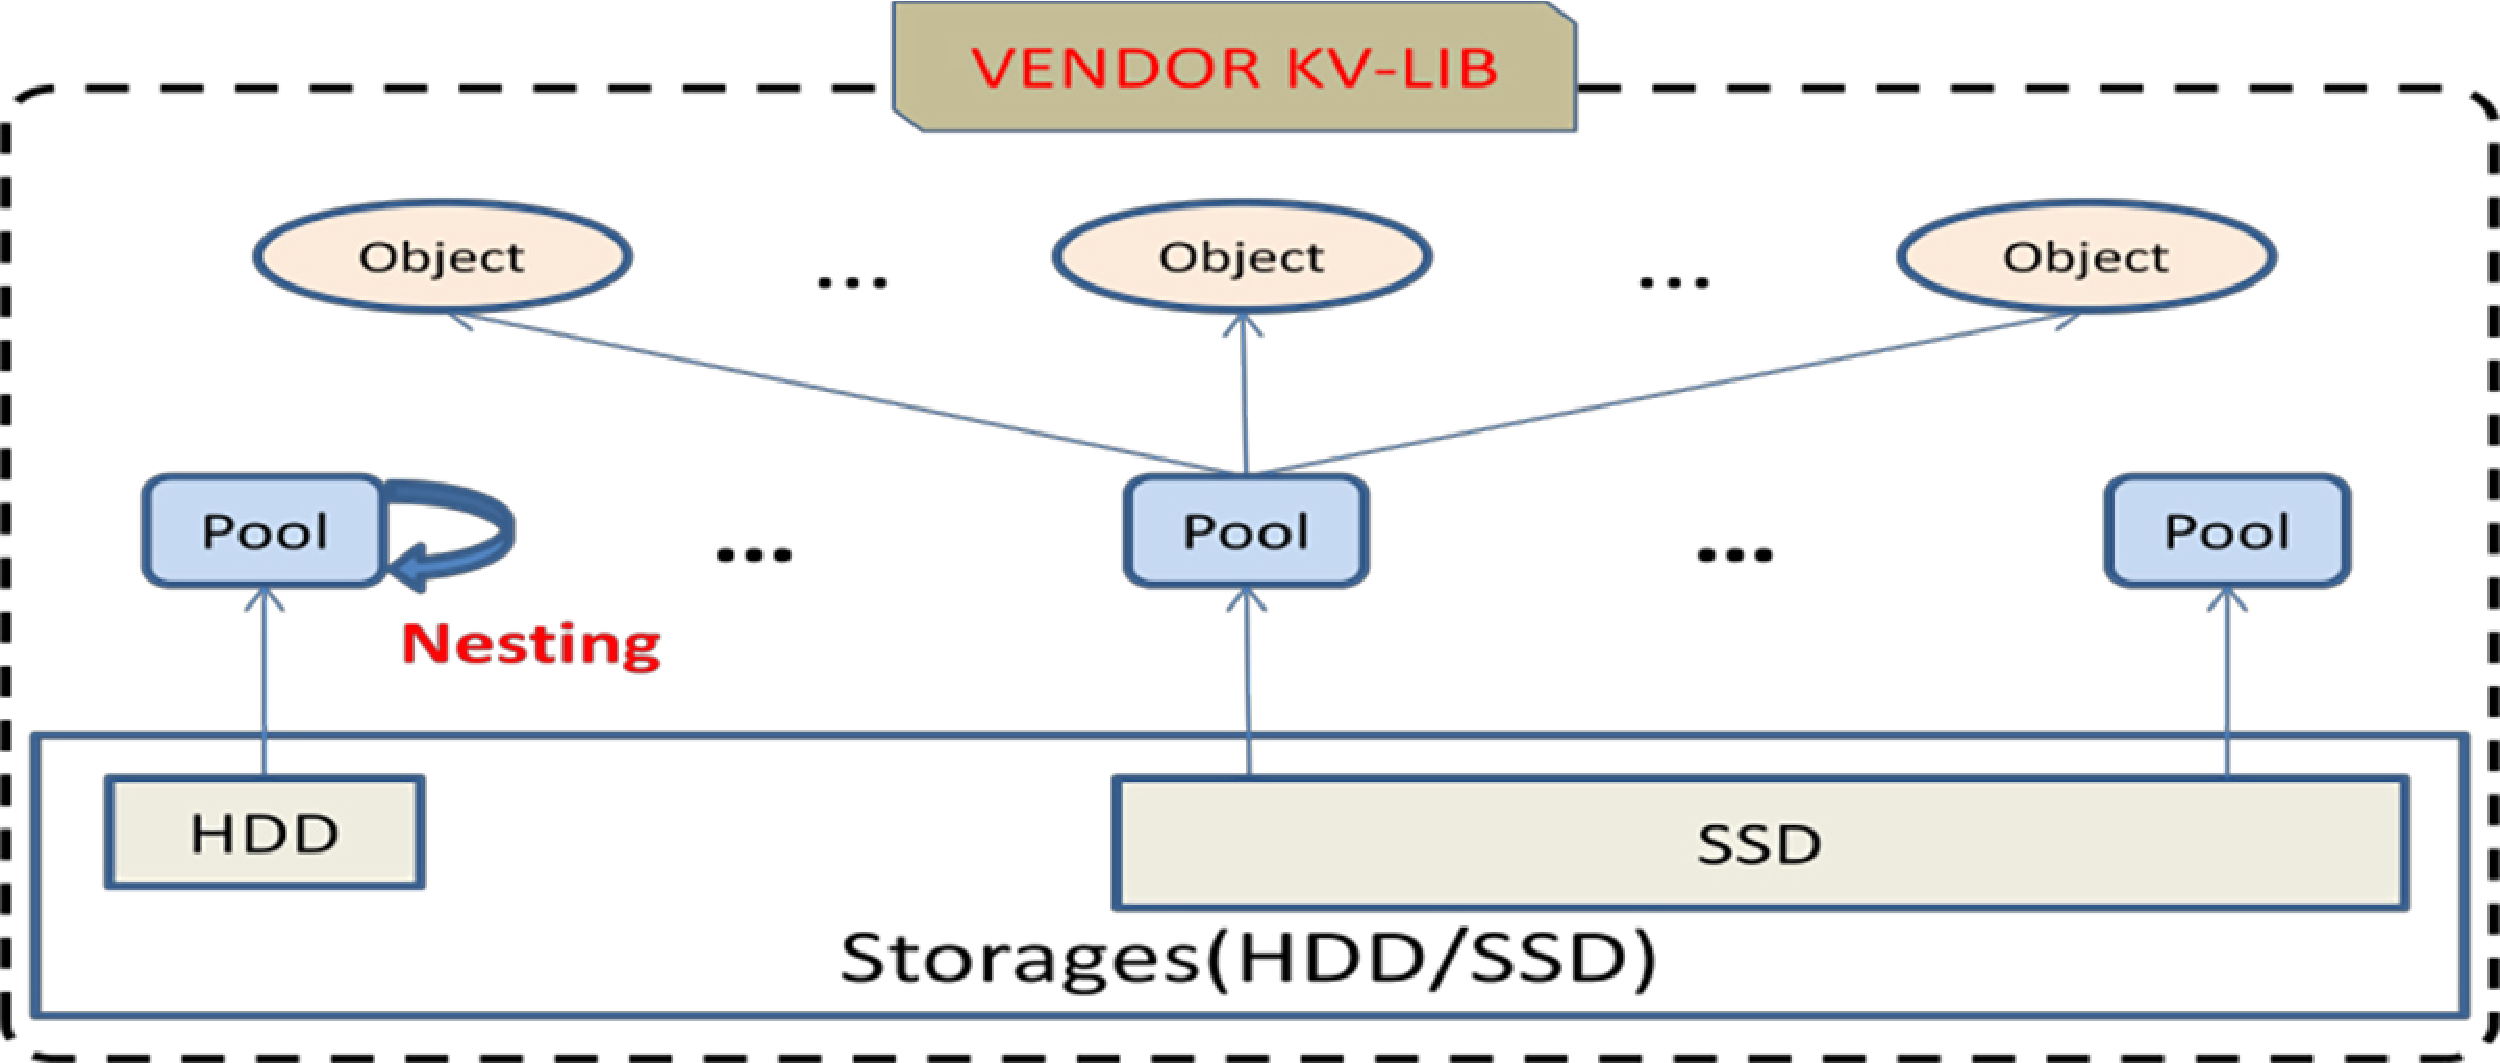
\includegraphics[width=13.9cm]{img/figure2.pdf}
	\end{center}
	\centerline {图2}

\section{Key Value Framework (KVF) 体系结构}\label{sec:KVF-Architecture}
	KVF提供了两层接口:底层管理接口(Lower Layer Manage API)和上层访问接口(Upper Layer Access API)。如图3所示
	\begin{center}
		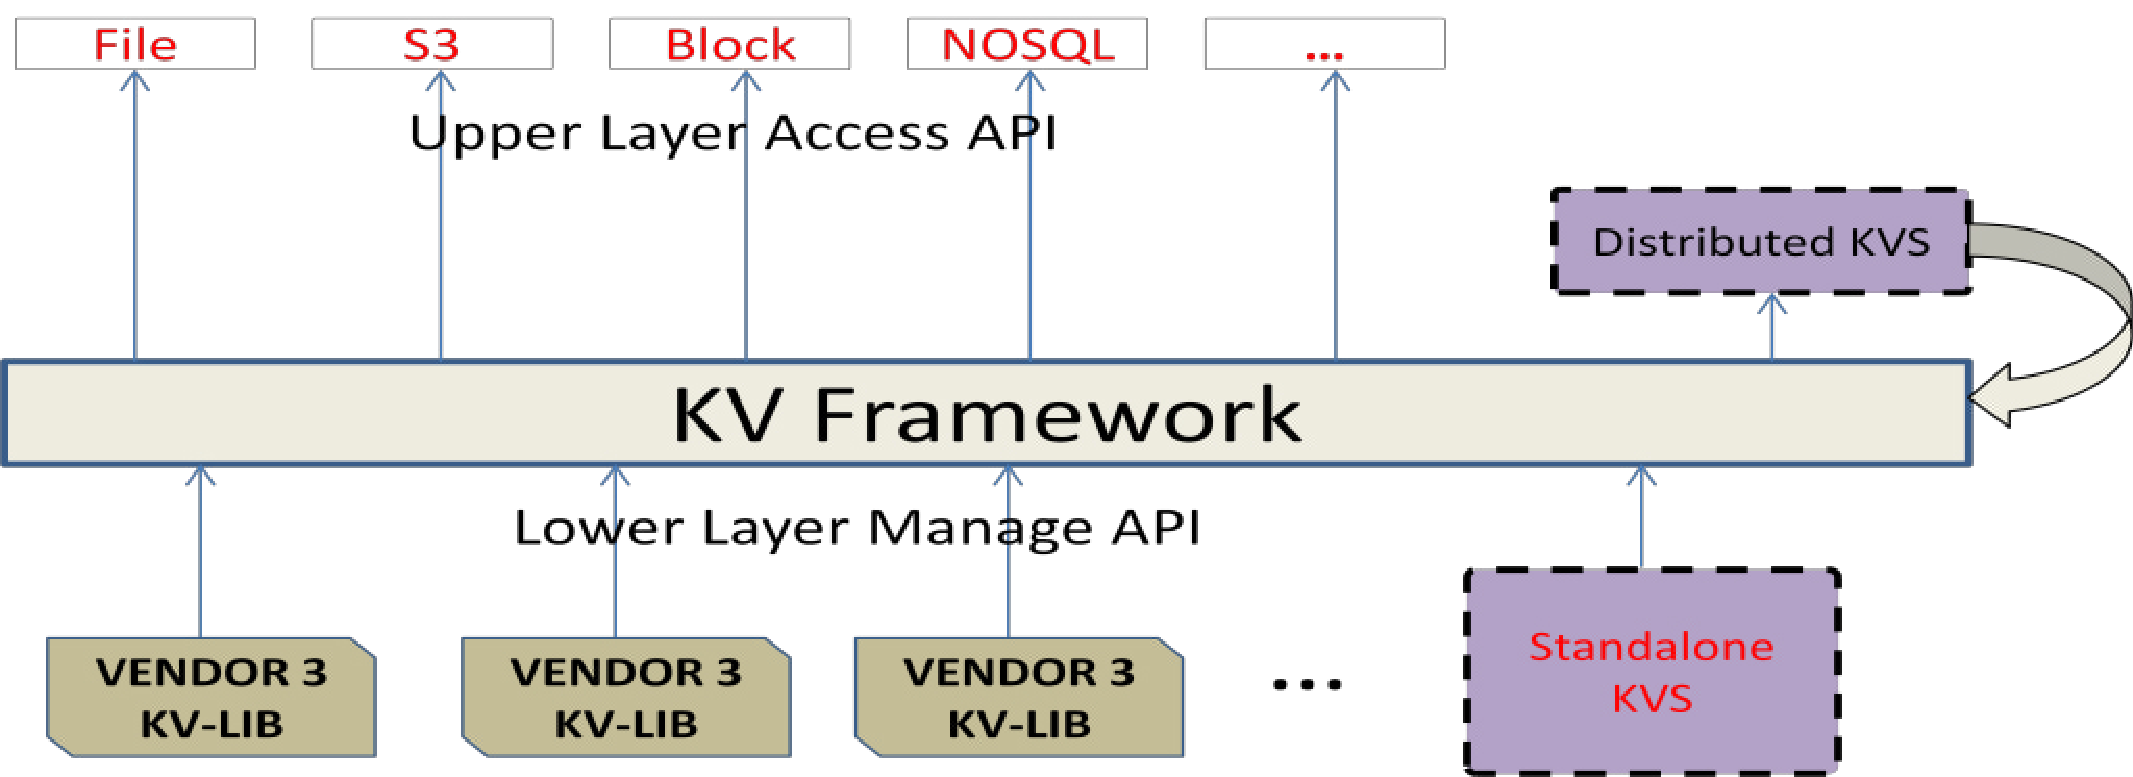
\includegraphics[width=13.9cm]{img/figure3.pdf}
	\end{center}
	\centerline {图3}
	底层管理提供注册和注销函数,共有三种接口:对象接口,Pool接口和KV-LIB接口。
	上层访问提供统一的键值接口,从而使上层应用程序变得简单并有更强的兼容性。
	此外一些应用可以通过利用基于其他KVS的上层访问接口提供键值服务,然后再重新注册到KVF中,这样就使得嵌套设计变得容易。
% \section{Key Value Framework (KVF) 底层管理接口}\label{sec:KVF-Lower-Layer-Manage-API}
% 	这节将描述底层管理接口设计,包括KVF接口,Pool接口,对象接口。KVF的相关函数名称都以“KVF\_”开始。
% 	\subsection{基本数据结构}
% 		基本数据类型定义
% 		\begin{center}
% 			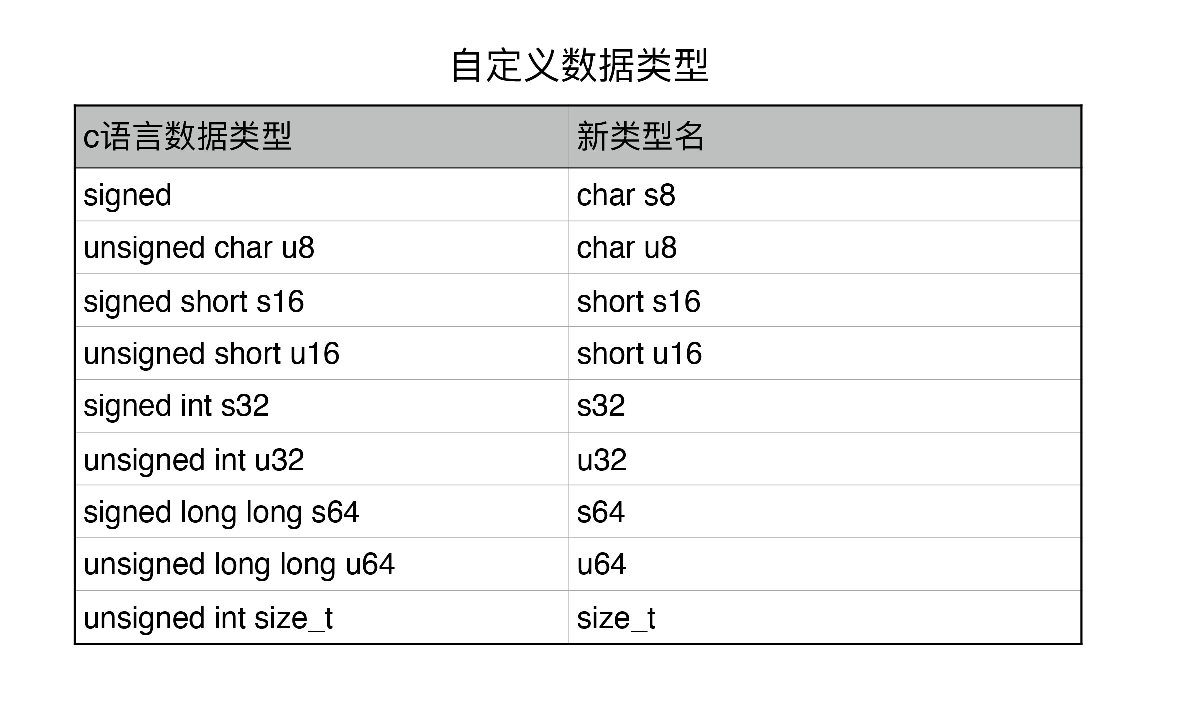
\includegraphics[width=13.9cm]{img/figure4.pdf}
% 		\end{center}

% 		字符串结构定义
% 		\begin{center}
% 			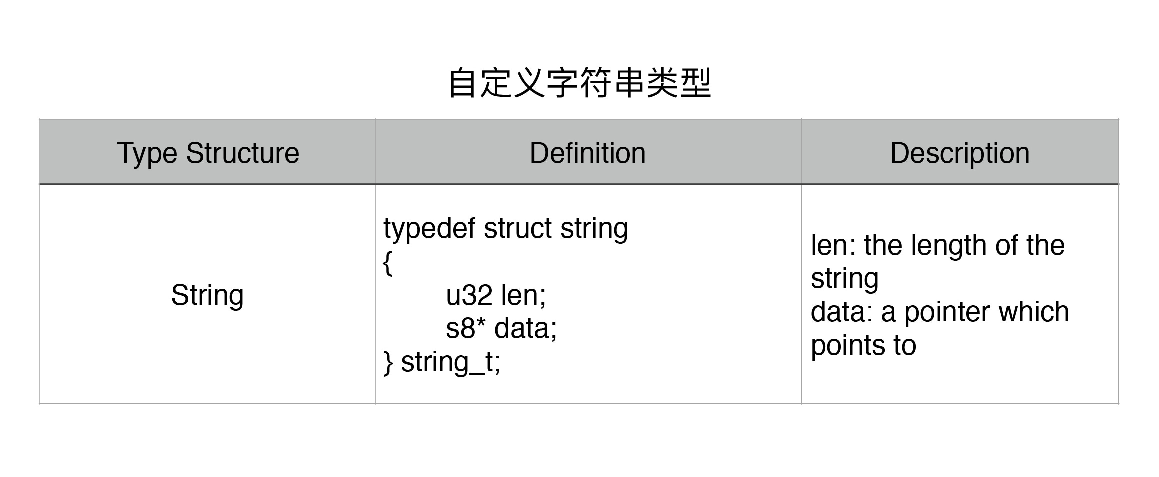
\includegraphics[width=13.9cm]{img/figure5.pdf}
% 		\end{center}




	% Copyright (c) 2014,2016 Casper Ti. Vector
% Public domain.
\chapter{KV Framework底层管理接口设计}
% \pkuthssffaq % 中文测试文字。
% vim:ts=4:sw=4
\section{概览}\label{sec:Overview}
	这章将描述底层管理接口设计,包括KVF接口,Pool接口,对象接口。KVF的相关函数名称都以“KVF\_”开始。
\section{基本数据结构}\label{sec:KVF-Basic-Data-Structure}
	
	\subsection{基本数据结构}
		\begin{center}
			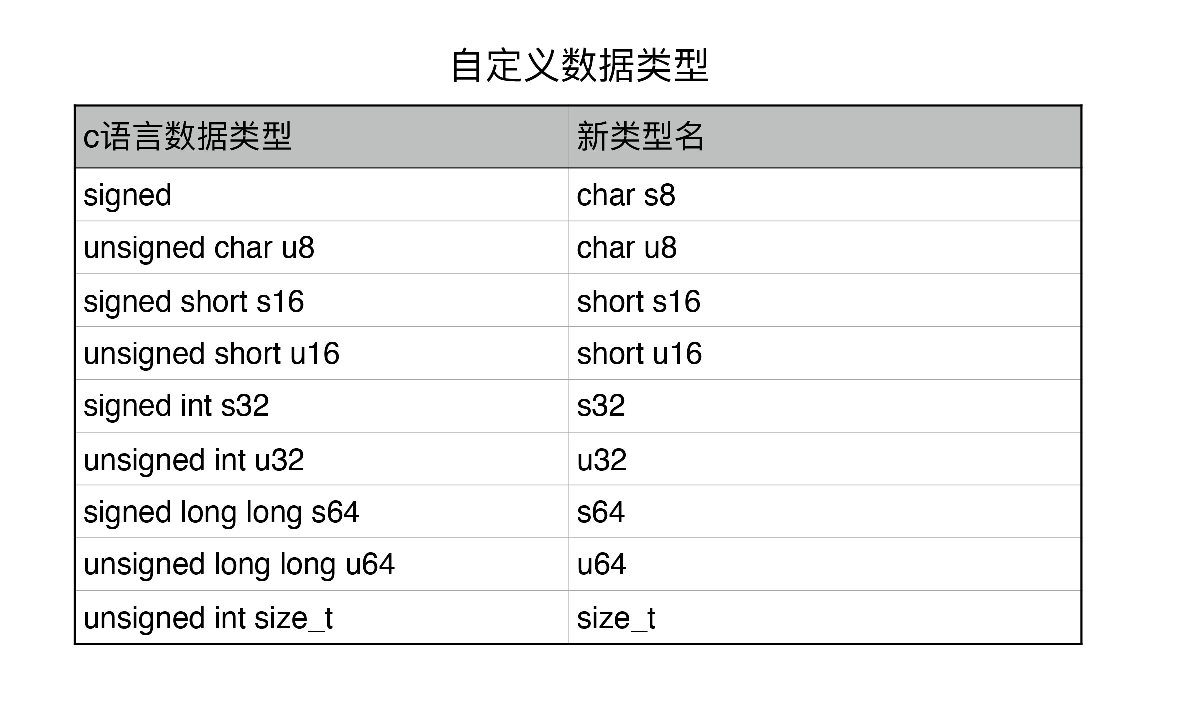
\includegraphics[width=13.9cm]{img/figure4.pdf}
		\end{center}
	\subsection{字符串结构定义}
		\begin{center}
			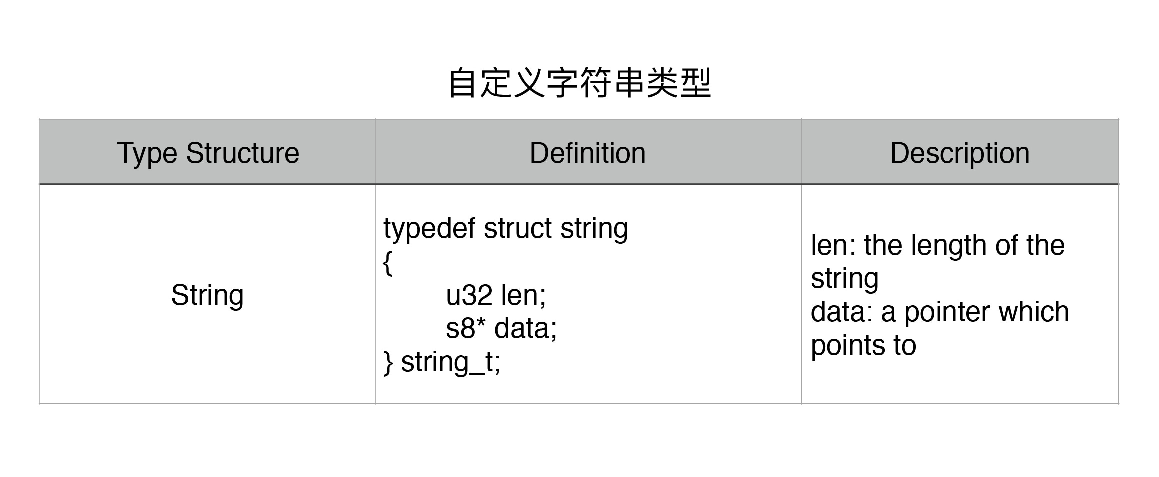
\includegraphics[width=13.9cm]{img/figure5.pdf}
		\end{center}

\section{KVF注册和注销接口}
	\begin{Verbatim}[frame = none]
    s32 kvf_register(kvf_type_t * kvf)
	\end{Verbatim}
	\begin{Verbatim}[frame = none]
    s32 kvf_unregister(kvf_type_t * kvf)
	\end{Verbatim}
		

	这两个接口使得厂商可以注册和注销自己的键值存储到KVF中,相关信息应该存储在kvf\_type\_t数据结构中,是开发者必须实现的函数。

	kvf\_type\_t结构定义如下

	\begin{center}
		\includegraphics[width=13.9cm]{img/figure6.pdf}
	\end{center}
\section{KV-LIB 接口}
	KV-LIB是厂商指定的键值库,通过这个键值库,厂商可以管理键值存储,包括初始化、关闭、设置属性等待。
	\subsection{kvf\_init()}
		该函数用于初始化KVF
		\begin{Verbatim}[frame = none]
    s32 kvf_init(const char * config_file)
		\end{Verbatim}

		参数说明:
			
			configure\_file:是指定的配置文件的目录
	\subsection{kvf\_shutdown ()}
		该函数用于关闭KVF
			
		\begin{Verbatim}[frame = none]
    s32 kvf_shutdown()
		\end{Verbatim}

		参数说明:
		\begin{itemize}
			\item \verb||
				此函数没有参数
		\end{itemize}
		% \begin{itemize}
		% 	\item \verb|copyright.tex|:版权声明部分。
		% 	\item \verb|originauth.tex|:
		% 		原创性声明和使用授权说明部分\supercite{pku-originauth}。
		% \end{itemize}

	\subsection{kvf\_set\_prop()}
		该函数用于设置KVF的相关属性值
		\begin{Verbatim}[frame = none]
    s32 kvf_set_prop(const char* name, const char* value)		
		\end{Verbatim}
		

		参数说明:
		\begin{itemize}
		\item \verb|name|:
			是指相关属性的名称
		\item \verb|value|:
			是相关属性的值
		\end{itemize}

	\subsection{kvf\_get\_prop()}
		该函数用于获得KVF的相关属性值
		\begin{Verbatim}[frame = none]
    s32 kvf_get_prop(const char* name, const char* value)		
		\end{Verbatim}
		

		参数说明:
		\begin{itemize}
		\item \verb|name|:
			是指相关属性的名称
		\item \verb|value|:
			是相关属性的值
		\end{itemize}
	
	\subsection{kvf\_alloc\_buf()}
		该函数用于在内存中分配一段数据缓冲区
		\begin{Verbatim}[frame = none]
    void* kvf_alloc_buf (size_t size, s32 flag)		
		\end{Verbatim}
		
		参数说明:
		\begin{itemize}
		\item \verb|size|:
			是需要的缓冲区空间大小
		\item \verb|flag|:
			是相关属性的值
		\end{itemize}
		
	\subsection{kvf\_free\_buf()}
		该函数用于在内存中释放数据缓冲区
		\begin{Verbatim}[frame = none]
    void* kvf_free_buf (void** buf)		
		\end{Verbatim}
		
		参数说明:
		\begin{itemize}
		\item \verb|buf|:
			需要释放内存空间的指针
		
		\end{itemize}
		
	\subsection{kvf\_get\_errstr()}
		该函数用于根据错误代码得到描述错误问题的字符串
		
		\begin{Verbatim}[frame = none]
    const char* kvf_get_errstr (s32 err_code)		
		\end{Verbatim}
		
		参数说明:
		\begin{itemize}
		\item \verb|err_code|:
			错误代码
		
		\end{itemize}

	\subsection{kvf\_get\_stats()}
		该函数u 用语获得KVF的统计数据

		\begin{Verbatim}[frame = none]
    s32 kvf_get_stats (kvf_stats_t* kvfstats)		
		\end{Verbatim}
		
		参数说明:
		\begin{itemize}
		\item \verb|kvfstats|:
			传入该kvf\_stats\_t结构的指针,函数体将数据写入该指针所指向的内存地址
		
		\end{itemize}

	% \subsection{kvf\_trans\_start()}
	% 	s32 kvf\_trans\_start(kv\_trans\_id\_t ** t\_id)
	% 	参数说明:
	% 		name是指相关参数的名词
	% 		value是相关参数的值
	% \subsection{kvf\_trans\_commit()}
	% 	s32 kvf\_trans\_commit(kvf\_trans\_id\_t* t\_id)
	% 	参数说明:
	% 		name是指相关参数的名词
	% 		value是相关参数的值
	% \subsection{kvf\_trans\_abort()}
	% 	s32 kvf\_trans\_abort(kvf\_trans\_id\_t* t\_id)
	% 	参数说明:
	% 		name是指相关参数的名词
	% 		value是相关参数的值

\section{POOL接口}
	在KVF-LIB注册并初始化之后,pool才能被管理。
	pool\_t的结构体定义如下:
	\begin{center}
		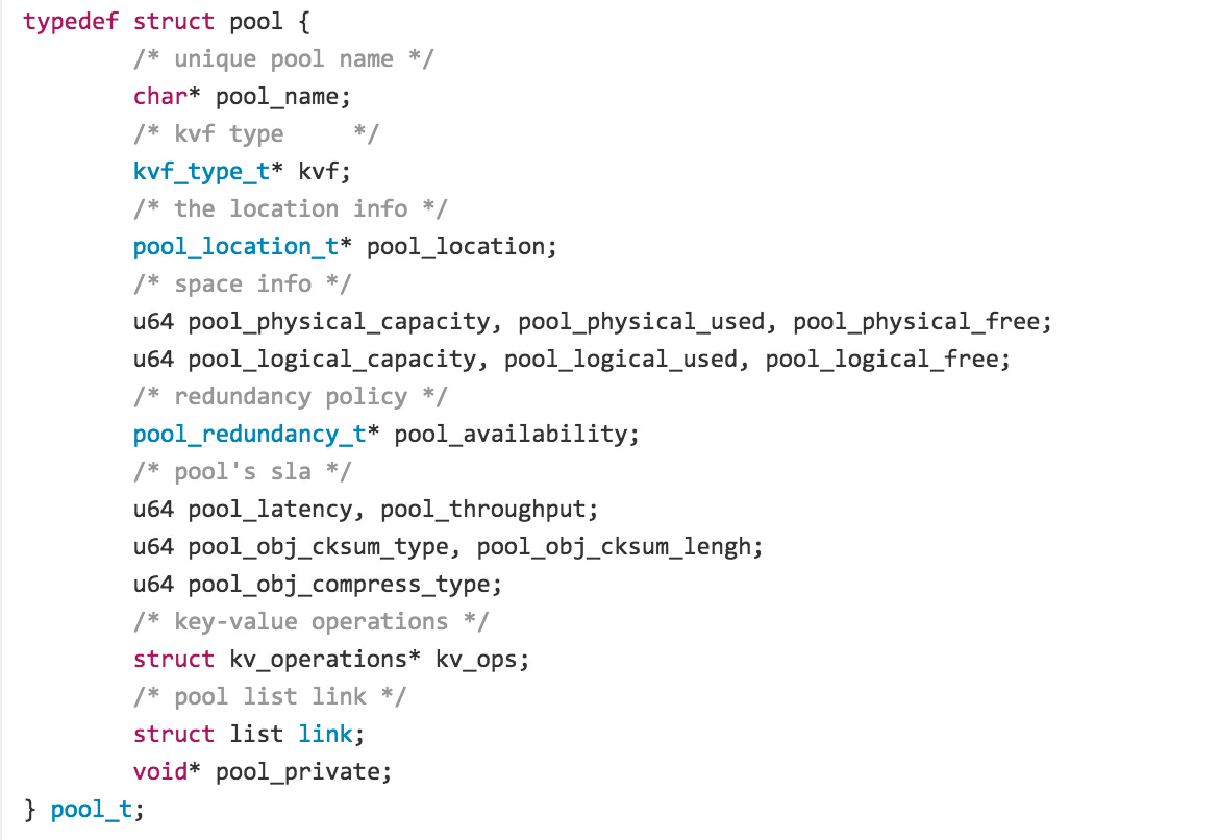
\includegraphics[width=13.9cm]{img/figure7.pdf}
	\end{center}
	\subsection{pool\_create()}
		用于创建新的pool
		\begin{Verbatim}[frame = none]
    s32 pool_create (const char* name, const char* config_path, 
		    pool_t * pool)	
		\end{Verbatim}

		参数说明:
		\begin{itemize}
		\item \verb|name|:
			指定pool的名称,每个KVF里的pool的name须唯一
		\item \verb|config_path|:
			指定相关配置文件的路径
		\item \verb|pool|:
			传入pool\_t结构指针,函数体将数据写入该指针所指向的内存地址		
		\end{itemize}
		

	\subsection{pool\_destroy()}
		销毁一个pool
		\begin{Verbatim}[frame = none]
    s32 pool_destroy (pool_t * pool)
		\end{Verbatim}

		参数说明:
		\begin{itemize}
		\item \verb|pool|:
			传入pool\_t结构指针,函数体将数据写入该指针所指向的内存地址
		\end{itemize}


	\subsection{pool\_open()}
		打开一个pool
		\begin{Verbatim}[frame = none]
    s32 pool_open (pool_t * pool)
		\end{Verbatim}		

		参数说明:
		\begin{itemize}
		\item \verb|pool|:
			传入pool\_t结构指针,函数体将数据写入该指针所指向的内存地址
		\end{itemize}


	\subsection{pool\_close()}
		关闭一个pool
		\begin{Verbatim}[frame = none]
    s32 pool_close (pool_t * pool)
		\end{Verbatim}		

		参数说明:
		\begin{itemize}
		\item \verb|pool|:
			传入pool\_t结构指针,函数体将数据写入该指针所指向的内存地址
		\end{itemize}


	\subsection{pool\_set\_prop()}
		设置pool的相关属性
		\begin{Verbatim}[frame = none]
    s32 pool_set_prop (const pool_t * pool,const char* name, 
			    const char* value )
		\end{Verbatim}

		参数说明:
		\begin{itemize}
		\item \verb|pool|:
			传入pool\_t结构指针,函数体将数据写入该指针所指向的内存地址,该参数是常量
		\item \verb|name|:
			需要设置的属性名称
		\item \verb|value|:
			需要设置的属性值
		\end{itemize}
	\subsection{pool\_get\_prop()}
		获取指定pool属性的值
		\begin{Verbatim}[frame = none]
    s32 pool_get_prop (const pool_t * pool,const char* name, 
			    const char* value )
		\end{Verbatim}

		参数说明:
		\begin{itemize}
		\item \verb|pool|:
			传入pool\_t结构指针,函数体将数据写入该指针所指向的内存地址,该属性是常量
		\item \verb|name|:
			需要设置的属性名称
		\item \verb|value|:
			需要设置的属性值
		\end{itemize}

	\subsection{pool\_get\_stats()}
		获取pool的统计数据
		\begin{Verbatim}[frame = none]
    s32 pool_set_stats (pool_stats_t * stats)
		\end{Verbatim}		

		参数说明:
		\begin{itemize}
		\item \verb|stats|:
			传入pool\_stats\_t结构指针,函数体将数据写入该指针所指向的内存地址
		\end{itemize}
	
	\section{对象键值接口}
		在pool成功创建之后,我们可以操作属于于该pool的对象

		\subsection{put}
			将数据写入磁盘
		\begin{Verbatim}[frame = none]
    s32 put(pool_t* pool,const string_t* key, const string_t* value,
	    const kv_props_t* props, const put_options_t* putopts)
		\end{Verbatim}

		参数说明:
		\begin{itemize}
		\item \verb|pool|:
			传入pool\_t结构指针,函数体将数据写入该指针所指向的内存地址,该参数是常量
		\item \verb|key|:
			需要写入的键
		\item \verb|value|:
			需要写入的属性值
		\item \verb|props|:
			设置键值的属性
		\item \verb|putopts|:
			设置写入模式
		\end{itemize}

		相关结构定义:
		\begin{center}
			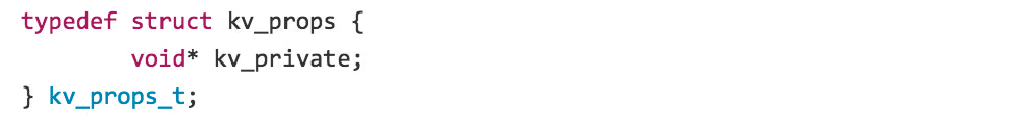
\includegraphics[width=13.9cm]{img/figure8.pdf}
		\end{center}
		\begin{center}
			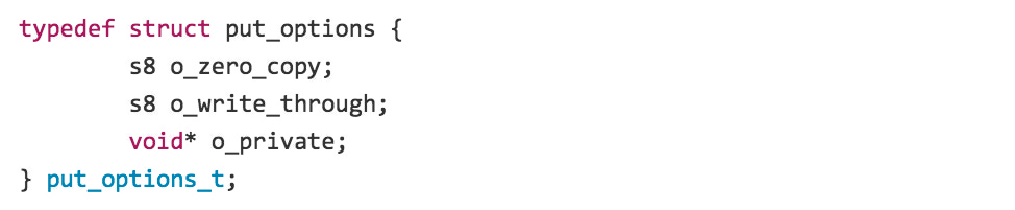
\includegraphics[width=13.9cm]{img/figure9.pdf}
		\end{center}


		\subsection{get}
			从磁盘中根据键获取值
		\begin{Verbatim}[frame = none]
    s32 get(pool_t* pool, const string_t* key, string_t* value, 
	    const kv_props_t* props, const get_options_t* getopts)
		\end{Verbatim}

		参数说明:
		\begin{itemize}
		\item \verb|pool|:
			传入pool\_t结构指针,函数体将数据写入该指针所指向的内存地址,该参数是常量
		\item \verb|key|:
			需要写入的键
		\item \verb|value|:
			该参数是string\_t结构指针,会将读取的值放入这个指针所指向的地址
		\item \verb|props|:
			设置键值的属性
		\item \verb|putopts|:
			设置写入模式
		\end{itemize}


		\subsection{del}
			从磁盘中根据键删除值
		\begin{Verbatim}[frame = none]
    s32 del(pool_t* pool, const string_t* key, const kv_props_t* props, 
        const del_options_t* delopts)
		\end{Verbatim}

		参数说明:
		\begin{itemize}
		\item \verb|pool|:
			传入pool\_t结构指针,函数体将数据写入该指针所指向的内存地址,该参数是常量
		\item \verb|key|:
			需要设置的属性名称
		\item \verb|value|:
			需要设置的属性值
		\item \verb|props|:
			设置键值的属性
		\item \verb|delopts|:
			设置写入模式
		\end{itemize}

		\subsection{iter\_open}
			根据正则表达式查询
		\begin{Verbatim}[frame = none]
    s32 iter_open(const pool_t* pool, const string_t* key_regex, 
        s32 limit, s32 timeout, kv_iter_t* it)
		\end{Verbatim}

		参数说明:
		\begin{itemize}
		\item \verb|pool|:
			传入pool\_t结构指针,函数体将数据写入该指针所指向的内存地址,该参数是常量
		\item \verb|key_regex|:
			需要查询的键的正则表达式
		\item \verb|limit|:
			查询次数的上限
		\item \verb|timeout|:
			timeout
		\item \verb|it|:
			
		\end{itemize}

		\subsection{iter\_next}
			根据正则表达式查询
		\begin{Verbatim}[frame = none]
    s32 iter_next(pool_t* pool, kv_iter_t* it, kv_array_t* kvarray)
		\end{Verbatim}

		参数说明:
		\begin{itemize}
		\item \verb|pool|:
			传入pool\_t结构指针,函数体将数据写入该指针所指向的内存地址,该参数是常量
		\item \verb|it|:
			需要查询的键的正则表达式
		\item \verb|kvarray|:
			查询次数的上限
		
		\end{itemize}

		\subsection{iter\_close}
			根据正则表达式查询
		\begin{Verbatim}[frame = none]
    s32 iter_close(pool_t* pool, kv_iter_t* it)
		\end{Verbatim}

		参数说明:
		\begin{itemize}
		\item \verb|pool|:
			传入pool\_t结构指针,函数体将数据写入该指针所指向的内存地址,该参数是常量
		\item \verb|it|:
			需要查询的键的正则表达式
		
		\end{itemize}

	\section{上层接口}
		当上层应用开发时调用如下的接口即可避免重发的适配工作,KVF将会封装常用的数据库,这样上层应用就不再考虑不同数据库之间接口的差异,大大缩短开发时间。

		根据不同的抽象层次,我们将接口分为三种:KV-LIB、Pool、对象。由于大部分功能和底层接口类似,在这里我将不再详细介绍每一个函数参数的含义。
		\subsection{KVF接口}

			\begin{Verbatim}[frame = none]
    s32 kvf_init(const char * config_file) 

    kvf_type_t* get_kvf(const char* name)

    s32 init_kvf(const char * config_file)

    s32 shutdown_kvf()

    s32 set_kvf_ prop(const char* name, const char* value)

    s32 get_kvf_ prop(const char* name, char** value)

    void* alloc_kvf_ buf (size_t size, s32 flag)

    void free_kvf_ buf (void** buf)

    s32 get_kvf_ stats (kvf_stats_t* kvfstats)

    s32 start_kvf_trans (kv_trans_id_t ** t_id)

    s32 commit_kvf_trans (kvf_trans_id_t* t_id)
    
    s32 abort_kvf_trans (kvf_trans_id_t* t_id)
			\end{Verbatim}

		\subsection{Pool接口}
			\begin{Verbatim}[frame = none]
    s32 create_pool (const char* name, const char* config_path, 
    pool_t * pool)

    s32 destroy_pool (pool_t * pool)

    s32 open_pool (pool_t * pool)

    s32 close_pool (pool_t* pool)

    s32 set_pool_prop(const pool_t* pool, const char* name, 
    const char* value )

    s32 get_pool_prop(const pool_t* pool, const char* name, 
    char** value)
    s32 get_pool_stats (pool_stats_t * stats)

			\end{Verbatim}

		\subsection{Pool接口}
			\begin{Verbatim}[frame = none]
    s32 put(pool_t* pool,const string_t* key, const string_t* value,
    const kv_props_t* props, const put_options_t* putopts);

    s32 get(pool_t* pool, const string_t* key, string_t* value, 
    const kv_props_t* props, const get_options_t* getopts)

    s32 del(pool_t* pool, const string_t* key, const kv_props_t* props, 
    const del_options_t* delopts)

    s32 mput(pool_t* pool, kv_array_t* kvarray, const kv_props_t* props, 
    const put_options_t* putopts)

    s32 mget(pool_t* pool, kv_array_t* kvarray, const kv_props_t* props, 
    const get_options_t* getopts)

    s32 mdel(pool_t* pool, array_t* kvarray, const kv_props_t* props, 
    const del_options_t* delopts)

    s32 open_iter (const pool_t* pool, const string_t* key_regex, 
    s32 limit, s32 timeout, kv_iter_t* it)

    s32 next_iter (pool_t* pool, kv_iter_t* it, 
    kv_array_t* kvarray)

    s32 close_iter (pool_t* pool, kv_iter_t* it)

    s32 xcopy_obj(const pool_t* src, const pool_t* dest,
    const string_t* regex)

			\end{Verbatim}
	\section{概览}\label{sec:Overview}
	YCSB(Yahoo! Cloud Serving Benchmark)是用来测试cloud serving/NoSQL/Key-Value Store的测试工具,代码开源,详细介绍见论文Benchmarking Cloud Serving Systems with YCSB。由于云服务的流行,传统数据库不能满足可利用性、可扩展性等要求,因此功能简化、一致性简化的NoSQL数据库逐渐流行。然而NoSQL数据库种类繁多,针对不同目的数据库各有权衡(读写性能、延迟和持久性、同步喝异步等等),用户和开发人员需要针对不同的应用场景选择合适的数据库。YCSB的目标是提供一个公平的平台,为这些数据库提供一个统一的测试方案,从而更公平地在不同的方面衡量不同的数据库性能,从而提供有价值的参考。

\section{YCSB应用模型}\label{sec:YCSB-Model}

	YCSB使用java编写,因为很多NoSQL系统拥有Java接口,其他没有Java接口的NoSQL系统可以通过比如HTTP/REST、JNI(Java Native Interface)等方式与java进行连接。由于KVF框架由c语言编写,所以在对KVF进行测试的时候需要用到JNI技术来实现KVF于YCSB的连接。

	YCSB模型图如下所示:

\begin{center}
	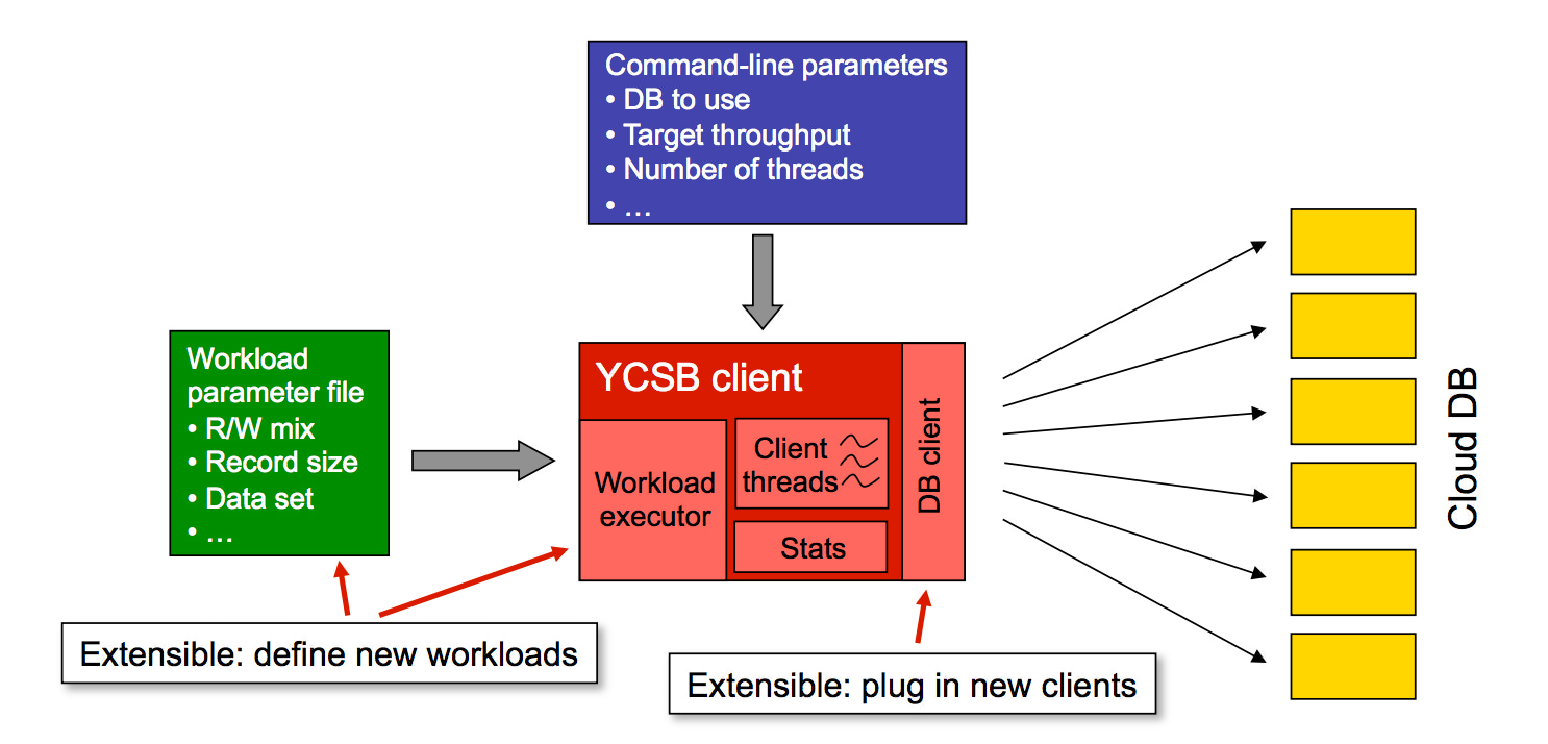
\includegraphics[width=13.9cm]{img/figure10.pdf}
\end{center}

	可以看出YCSB系统可以分为四个部分,分别是YCSB客户端,云数据库,任务集和命令行参数。

	\subsection{YCSB客户端}
		YCSB客户端是整个系统的核心,它包括任务集执行器,客户端线程,统计数据,和数据库客户端。

		YCSB客户端是一个用来产生数据和操作的Java程序,数据用来被加载到数据库中,操作包括读写更新删除等等,这些操作构成了任务集。基本的运行流程是任务集执行器驱动多个客户端线程,每一个线程执行一系列的操作,这些操作被标记为数据库接口层的调用,包括加载数据库(加载阶段)和执行任务集(交易阶段)。这些线程可以自行调节它们所产生的不同请求的比例,因此我们通过直接编写workload的方式来控制它。这些线程还会测量延迟和这些操作实现的吞吐量,并将这个测量数据报告到统计数据模块中,在每一次实验的结束,统计数据模块负责整合测量数据病报告前95\%的延迟和99\%的延迟。

		客户端将用一系列的属性(属性名/值对)来定义它的操作。通常情况下,我们将这些属性分为两组:
		\begin{itemize}
			\item \textbf{任务集属性}:
		用来定义任务集的一系列属性,独立于一个给定的数据库或者实验运行。比如指定对数据库读写操作的混合比例,指定分布方式,和记录的数量、大小和域的数目等等。
			\item \textbf{运行时属性}:
		是针对于一个给定的实验的属性集合,比如指定哪一种数据库(比如Cassandra、HBase等),指定初始化接口层的属性(比如数据库服务的主机名),指定客户端线程的数量等等。

		\end{itemize}
		
		因此任务集属性文件可以是静态的,并被应用于不同的不同数据库的测试实验中,运行时属性也一样可以存储在属性文件中,但是真对不通的实验、数据库和目标吞吐量这些属性的值可能会大有不同。

	\subsection{Workload}
		workload指的是测试数据库系统时需要完成的任务集,在YCSB系统中自带六个workload,分别针对不用的应用场景

		Workload A: 更新操作权重很高的任务集

				这个任务集是由50\%的读操作和50\%的写操作混合而成,一个典型的应用例子是会话存储记录最近的行为。

		Workload B: 几乎全是读操作的任务集

				这个任务集由95\%的读操作和5\%的写操作混合而成,应用场景为照片打标签,添加标签是更新操作,但是绝大部分的操作是读取tag

		Workload C: 全部是读写的任务集

				这个任务集100\%是读,应用例子是用户简介的缓存,用户的简介实际上是在其他地方创建的。

		Workload D: 读最近的任务集

				在这个任务集中,新的记录被插入,最新插入的记录是最经常被读取的。一个典型的应用例子:用户更新,其他用户想要看到的是最新修改的内容。

		Workload E: 短的排列

				在这个任务集中,一小排记录被查询,而不是一个单独的记录,应用例子:一段对话,每一次扫描

		Workload F: 读-修改-写

				在这个任务集中,客户端将读一个记录,修改它,然后写回。应用例子:用户数据库,用户读取自己的记录然后

	\subsection{JNI}
		The Java Native Interface (JNI) 是一个Java软件开发工具的一个原声编程接口,通过它可以使得Java代码使用其他语言编写的代码和代码库,比如C和C++。 Invocation 接口是JNI的一部分,可以用来讲Java虚拟机(JVM)嵌入到原生应用中国年,从而允许其他语言的原生应用可以调用Java代码。

		在benchmarkd实现的过程中,需要以下工具:

		Java编译器:javac执行命令需要SDK

		Java虚拟机:java执行命令需要SDK

		原生方法C文件产生器:javah命令需要SDK

		定义了JNI的库文件和原生头文件:C头文件jni.h、jvm.lib、jvm.dll或者jvm.so都需要SDK

		可以产生共享库的C和C++编译器:在linux系统下cc编译器是最常见的

		在Java 2 SDK中,Java虚拟机和Java运行时支持位于共享库中的libjvm.so

		连接YCSB和KVF需要如下六步:

		编写Java代码。我们需要首先编写Java类来完成三个任务:声明将要调用的原生方法,加载包含原生代码的共享库,调用原生方法。

		编译Java代码。在使用之前我们必须成功将Java类编译成为二进制代码。

		创建C头文件。头文件中声明我们想调用的原生函数,这个头文件将用来和C函数实现一起创建共享库。

		写C代码,这一步需要实现C源代码,该文件必须包含在第三步创建的头文件。

		创建共享库文件。我们将从第4步获得的C源代码文件创建共享库文件。

		运行Java程序。

		为了对比KVF底层接于nvmkv后的功能和性能,我分别编写了Makefile来对KVF和nvmkv进行基本的测试,Makefile的实际上是指定了编译规则以及依赖关系,在每一个编译指令的最开始会指定生成对象的名称,然后指定生成该文件所依赖的文件名,在第二行指定编译工具以及编译细节,在编写Makefile时需要将最后编译的文件在最前面指出,因此整个Makefile的罗列顺序和实际的编译顺序是相反的。如下代码是列出了测试nvmkv时Makefile中关键的步骤,我将按照实际的编译顺序进行介绍。

		\begin{Verbatim}[frame = single]
	com/yahoo/ycsb/db/JNvmkv.class : com/yahoo/ycsb/db/JNvmkv.java
    javac com/yahoo/ycsb/db/JNvmkv.java

		\end{Verbatim}
		首先编译JNvmvk对象,这个类对nvmkv的底层函数进行了封装,供YCSB client调用。


		\begin{Verbatim}[frame = single]
	com/yahoo/ycsb/db/com_yahoo_ycsb_db_JNvmkv.h \ 
	com/yahoo/ycsb/db/JNvmkv.class
    javah -classpath . -d ./com/yahoo/ycsb/db/ \ 
        com.yahoo.ycsb.db.JNvmkv

		\end{Verbatim}
		这一步生成负荷JNI格式的头文件,其中每一个函数名都以com\_yahoo\_ycsb\_db\_开头,在编写Jnvmkv.c文件时,函数名要和这里的保持一致。



		\begin{Verbatim}[frame = single]
com.yahoo.ycsb.db.com_yahoo_ycsb_db_JNvmkv.o : \ 
	com/yahoo/ycsb/db/JNvmkv.c \ 
	com/yahoo/ycsb/db/nvmkv-test.h
    g++ -c $< -o com/yahoo/ycsb/db/com_yahoo_ycsb_db_JNvmkv.o\ 
        $(LDFLAGS) -I/usr/lib/jvm/java/include/ -I/usr/lib/jvm/\ 
        java/include/linux/ -fPIC
		
		\end{Verbatim}
		这一步生成目标文件,用于最终生成共享函数库文件。


		\begin{Verbatim}[frame = single]
com.yahoo.ycsb.db.libcom_yahoo_ycsb_db_JNvmkv.so : \ 
	com/yahoo/ycsb/db/com_yahoo_ycsb_db_JNvmkv.h : \
	com.yahoo.ycsb.db.com_yahoo_ycsb_db_JNvmkv.o
    gcc -I/usr/lib/jvm/java/include/\
        -I/usr/lib/jvm/java/include/linux/ \
        -L$(PATH_TO_ANANAS_LIB) $(LDLIBS) $(LDFLAGS)\
        -fPIC -o com/yahoo/ycsb/db/libcom_yahoo_ycsb_db_JNvmkv.so\ 
        -shared -Wl,-soname,com/yahoo/ycsb/db/\
        com_yahoo_ycsb_db_JNvmkv.so com/yahoo/ycsb/db/\
        com_yahoo_ycsb_db_JNvmkv.o
    javah -classpath . -d ./com/yahoo/ycsb/db/ \ 
        com.yahoo.ycsb.db.JNvmkv

		\end{Verbatim}
		这一步最终生成YCSB Client在运行时会调用的共享函数库文件。

		\begin{Verbatim}[frame = single]
run :
        java -Djava.library.path=$(PATH_TO_YCSB)YCSB/nvmkv/src/\
        main/java/com/yahoo/ycsb/db/\
        com.yahoo.ycsb.db.JNvmkv
		
		\end{Verbatim}
		在最终使用YCSB测试之前,我做了一个单独的基本功能测试,在运行时需要指定库文件路径,一遍调用上一步编译出来的共享函数库文件。

	\subsection{实现方式}
		YCSB是一套完整的测试系统,我们需要将KVF当作YCSB的一个数据库模块添加到YCSB中。YCSB的数据库接口层隐藏了所在做测试的NoSQL数据库的细节,这就允许客户端产生像“读记录”“更新记录”这样简单的操作,而不用理解你所指定数据库的特定接口。因此,YCSB很容易来测评一个新加入的数据库系统。一旦你创建了数据库接口层,YCSB框架的其他地方不需要做任何改变就可以顺利运行。

		YCSB的数据库接口层是一个简单的抽象类,为你的数据库提供了读、插入、更新、删除和扫描操作。为KVF实现一个数据库接口层只需要实现这具体的函数体,一旦这个接口层可以顺利编译,我们就可以在命令行(或者属性文件中)指定为KVF实现的类名。因此我们并不需要因为添加或者更改了数据库接口耳重新编译YCSB客户端。

		根据下列步骤即可完成KVF模块的创建

		\begin{Verbatim}[frame = none]
    第一步:继承 com.yahoo.ycsb.DB		
		\end{Verbatim}

		该类是所有数据库接口层实现的基类,它是一个抽象类,所以我们需要实现一个继承于com.yahoo.ycsb.DB的类,在这类我们把这个类声明为AnanasClient,这个类需要拥有一个无参数的构造函数,因为在AnanasClient的实例将会在YCSB内部通过无参数的构造函数生成。

		YCSB客户端框架会为AnanasClient的每一个线程都创建一个实例,但是我们需要测试多线程的功能,所以会有多个工作者线程都产生任务集,每一个线程都会创建一个AnanasClient实例。

		\begin{Verbatim}[frame = none]
    第二步:实现init()如果有必要的话
		\end{Verbatim}
		
		通过下面的方法我们可以初始化我们的DB对象:

		public void init() throws DBException

		该方法在每个AnanasClient实例中都会被调用一次,所以如果在测试的时候使用多线程的方式,每个AnanasClient实例都会被各调用一次。

		init()方法应该被用来连接数据库和其他相关初始化工作。需要指出的是,YCSB提供了一种可以在运行时使用属性文件配置数据库的方式。事实上,YCSB客户端会在启动的时候将在属性文件指定的所有参数文件都传递到数据库接口层。因此,我们可以为数据库接口层创建新的属性文件来,在参数文件中或者命令行中进行设置,然后在我们自己实现的AnanasClient中获得这个参数文件并设置相应的属性。

		这些属性将会在构造函数被调用后传递到实例中,因此我们需要在init()方法中获得这些属性而不是在构造函数中,我们可以调用下列方法,该方法已经被实现并从DB基类继承而来。


		\begin{Verbatim}[frame = none]
    第三步:实现数据库查询更新方法
		\end{Verbatim}

		下列方法是AnanasClient需要实现的:

		\begin{Verbatim}[frame = single]
  //Read a single record
  public int read(String table, String key, Set<String> fields, 
  HashMap<String,String> result);

  //Perform a range scan
  public int scan(String table, String startkey, int recordcount, 
  Set<String> fields, Vector<HashMap<String,String>> result);
	
  //Update a single record
  public int update(String table, String key, HashMap<String,
  String> values);

  //Insert a single record
  public int insert(String table, String key, HashMap<String,
  String> values);

  //Delete a single record
  public int delete(String table, String key);

		\end{Verbatim}
		在每一次调用的时候,这些方法都会使用一个表名称和记录的键。对于读和扫描方法,需要额外外的参数来提供一个数据结构存储返回的数据。对于插入和更行方法来说,需要传入映射了域名和值的哈西映射(HashMap)。

		数据库应该在运行测评之前创建号合适的表。我们在实现上述方法的时候认为适当的表已经存在,只需要从指定的表中读和写。

		在这里我将介绍KVF对应的YCSB Client的实现细节。
\begin{center}
	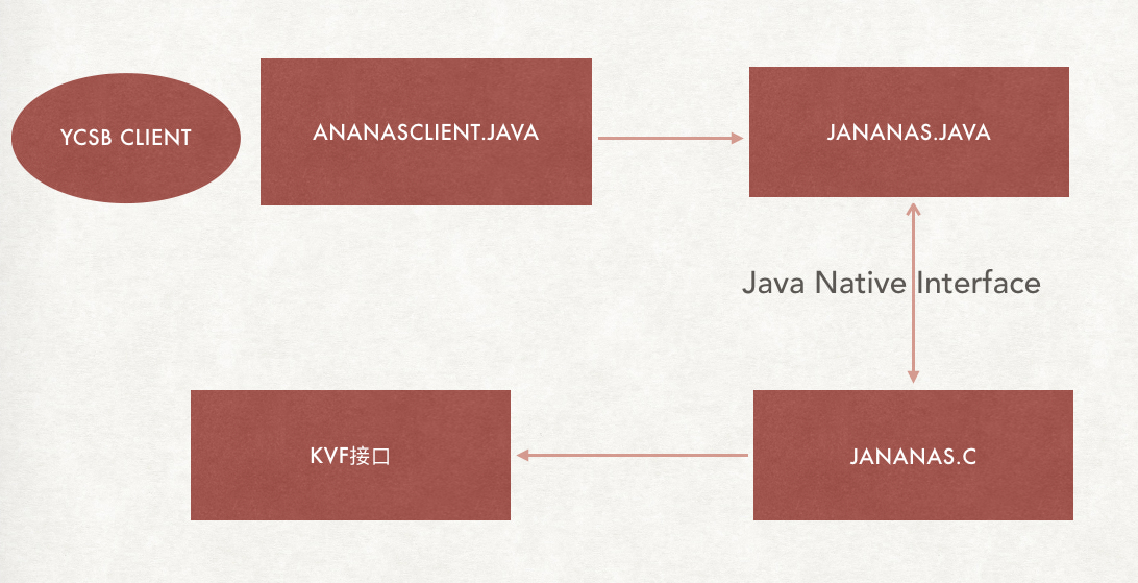
\includegraphics[width=13.9cm]{img/figure11.pdf}
\end{center}
		
		如上图所示,JAnanasClient是一个YCSB Client的实例,它继承了com.yahoo.ycsb.DB类,并实现了需要实现的函数,在实现的过程中使用JAnanas类进行具体的对数据库的操作,JAnanas类将KVF封装成为一个数据库,并通过JNI与JAnanas.c进行连接,从而调用KVF中实现的接口,达到访问数据库的目的。		

		\begin{Verbatim}[frame = none]
    第四步:编译数据库接口层
		\end{Verbatim}

		我们的代码可以独立于YCSB客户端和YCSB框架单独编译,因此当我们对自己的数据库接口层AnanasClient作修改之后只需编译自己的模块而不用重新编译YCSB客户端。


		\begin{Verbatim}[frame = none]
    第五步 测试数据库	
		\end{Verbatim}

		YCSB提供了简单的命令行客户端来测试接口层,它创建一个数据库实例,允许你世界操作数据库而不用启动一个任务集,例子如下:

\begin{Verbatim}[frame = single]

% java com.yahoo.ycsb.CommandLine -db com.yahoo.ycsb.db.MongoDbClient 
-p mongodb.url=mongodb://localhost:27017 -p mongodb.database=ycsb

YCSB Command Line client
Type “help” for command line help
Start with “-help” for usage info
Connected.
> insert brianfrankcooper first=brian last=cooper
Return code: 1
191 ms
> read brianfrankcooper
Return code: 0
last=cooper
_id=brianfrankcooper
first=brian
2 ms
> quit
\end{Verbatim}

		首先使用命令行工具以及相关的参数启动一个数据库,然后进行单独的插入、读、更新、删除等操作,这样即可自行验证功能的正确性。比如在上述实例中,首先插入一条记录,id为brianfrankcooper,第一个值为brian,第二个值为cooper,然后读取记录,读出的信息和插入的一样,验证成功。


		\begin{Verbatim}[frame = none]
	第六步:使用YCSB客户端测试
		\end{Verbatim}

		使用YCSB集成测试需要在YCSB项目的根目录下运行ycsb的python脚本,在命令行指定数据库和任务集以及线程等相关信息。

	\subsection{实现流程}

	1.在YCSB中新建一个文件kvf/,将KVF作为一个新的Database添加到YCSB框架中

	2.在YCSB/kvf/目录下新建pom.xml文件用于编译,文件内容和YCSB中其他database的相应文件一样,只需做与kvf相关的修改即可

	3.在YCSB/kvf/目录下仿照其他database的目录结构新建src/main/java/,在这个目录下创建Makefile用于简化编译过程

	4.在YCSB/kvf/src/main/java目录下新建com/yahoo/ycsb/db/目录结构,实现java的包结构方便进行编译

	5.在这个目录下新建文件AnanasClient.java,该类继承了com.yahoo.ycsb.DB类,在该类中重写了一些关键的方法来供YCSB的上层测试函数的调用

	6.创建JAnanas.java用于对kvf的包装

		因为kvf用c语言编写,YCSB为java编写,所以需要使用Java Native Interface来将其连接

	7.通过JAnanas.java编译出头文件com\_yahoo\_ycsb\_db\_JAnanas.h

	根据编译出的头文件编写com\_yahoo\_ycsb\_db\_JAnanas.c实现JAnanas.java中的native函数

	8.在YCSB/bin中的ycsb脚本文件第75行添加kvf

	9.在YCSB/pom.xml中添加kvf

	10.在distribution/pom.xml中添加kvf

	\subsection{测试计划}
	在图形界面客户端中进行测试
	对多线程进行测试:将线程数分别设置为1,2,4,8,16,21,64,128分别测试
。

	通过参数设置配置不同读、插入、更新、删除操作比例的测试文件进行测试:例如:不同读写比率(100\%插入、90\% 更新+ 10\%读、65\%读+25\% 插入+10\% 更新、90\% 读+10\% 插入、100\%读等)

	如下我可以自定义任务集,指定操作数、插入、更新、读取、删除的比例,以及分布方式:
\begin{Verbatim}[frame = single]
    workload=com.yahoo.ycsb.workloads.CoreWorkload
    readallfields=false
    readproportion=0.65
    updateproportion=0.25
    scanproportion=0
    insertproportion=0.1
    requestdistribution=uniform
\end{Verbatim}

	在这个任务集中首先会将1000个记录加载到数据库中,在实际测试的时候将有2000次操作,读取数据的比例是65\%,更新的比例为25\%,插入的比例为10\%,分布方式为全部随机分布,在命令行中指定线程数为16.

	通过YCSB的stat结构统计数据,我们可以得到如下的测试结果:

\begin{Verbatim}[frame = single]
[OVERALL], RunTime(ms), 516.0
[OVERALL], Throughput(ops/sec), 3875.968992248062
[CLEANUP], Operations, 1.0
[CLEANUP], AverageLatency(us), 5.0
[CLEANUP], MinLatency(us), 5.0
[CLEANUP], MaxLatency(us), 5.0
[CLEANUP], 95thPercentileLatency(us), 5.0
[CLEANUP], 99thPercentileLatency(us), 5.0
[INSERT], Operations, 216.0
[INSERT], AverageLatency(us), 554.5185185185185
[INSERT], MinLatency(us), 283.0
[INSERT], MaxLatency(us), 1852.0
[INSERT], 95thPercentileLatency(us), 961.0
[INSERT], 99thPercentileLatency(us), 1554.0
[INSERT], Return=0, 216
[READ], Operations, 1302.0
[READ], AverageLatency(us), 89.02150537634408
[READ], MinLatency(us), 34.0
[READ], MaxLatency(us), 701.0
[READ], 95thPercentileLatency(us), 206.0
[READ], 99thPercentileLatency(us), 288.0
[READ], Return=0, 1302
[UPDATE], Operations, 482.0
[UPDATE], AverageLatency(us), 143.00829875518673
[UPDATE], MinLatency(us), 69.0
[UPDATE], MaxLatency(us), 841.0
[UPDATE], 95thPercentileLatency(us), 236.0
[UPDATE], 99thPercentileLatency(us), 298.0
[UPDATE], Return=0, 482
\end{Verbatim}

	从结果中我们可以看到,吞吐量为3875.96op\/s,由于有16个线程所以会清除16次。

	插入操作有216次,平均延迟为554.51us,最大一次延迟为1852.0us,最小的一次延迟为283.0us,99\%的插入延迟在1554.0us以内,95\%的插入延迟在961.0us\%以内。

	读操作有1302次,平均延迟为89.02us,最大一次延迟为701.0us,最小的一次延迟为34.0us,99\%的读延迟在288.0us以内,95\%的读延迟在206.0us\%以内。


	更新操作有482次,平均延迟为143.00us,最大一次延迟为841.0us,最小的一次延迟为69.0us,99\%的读延迟在298.0us以内,95\%的读延迟在236.0us\%以内。

	为了更近直观地分析和对比数据,我将YCSB的测试结构进行可视化处理。

\begin{center}
	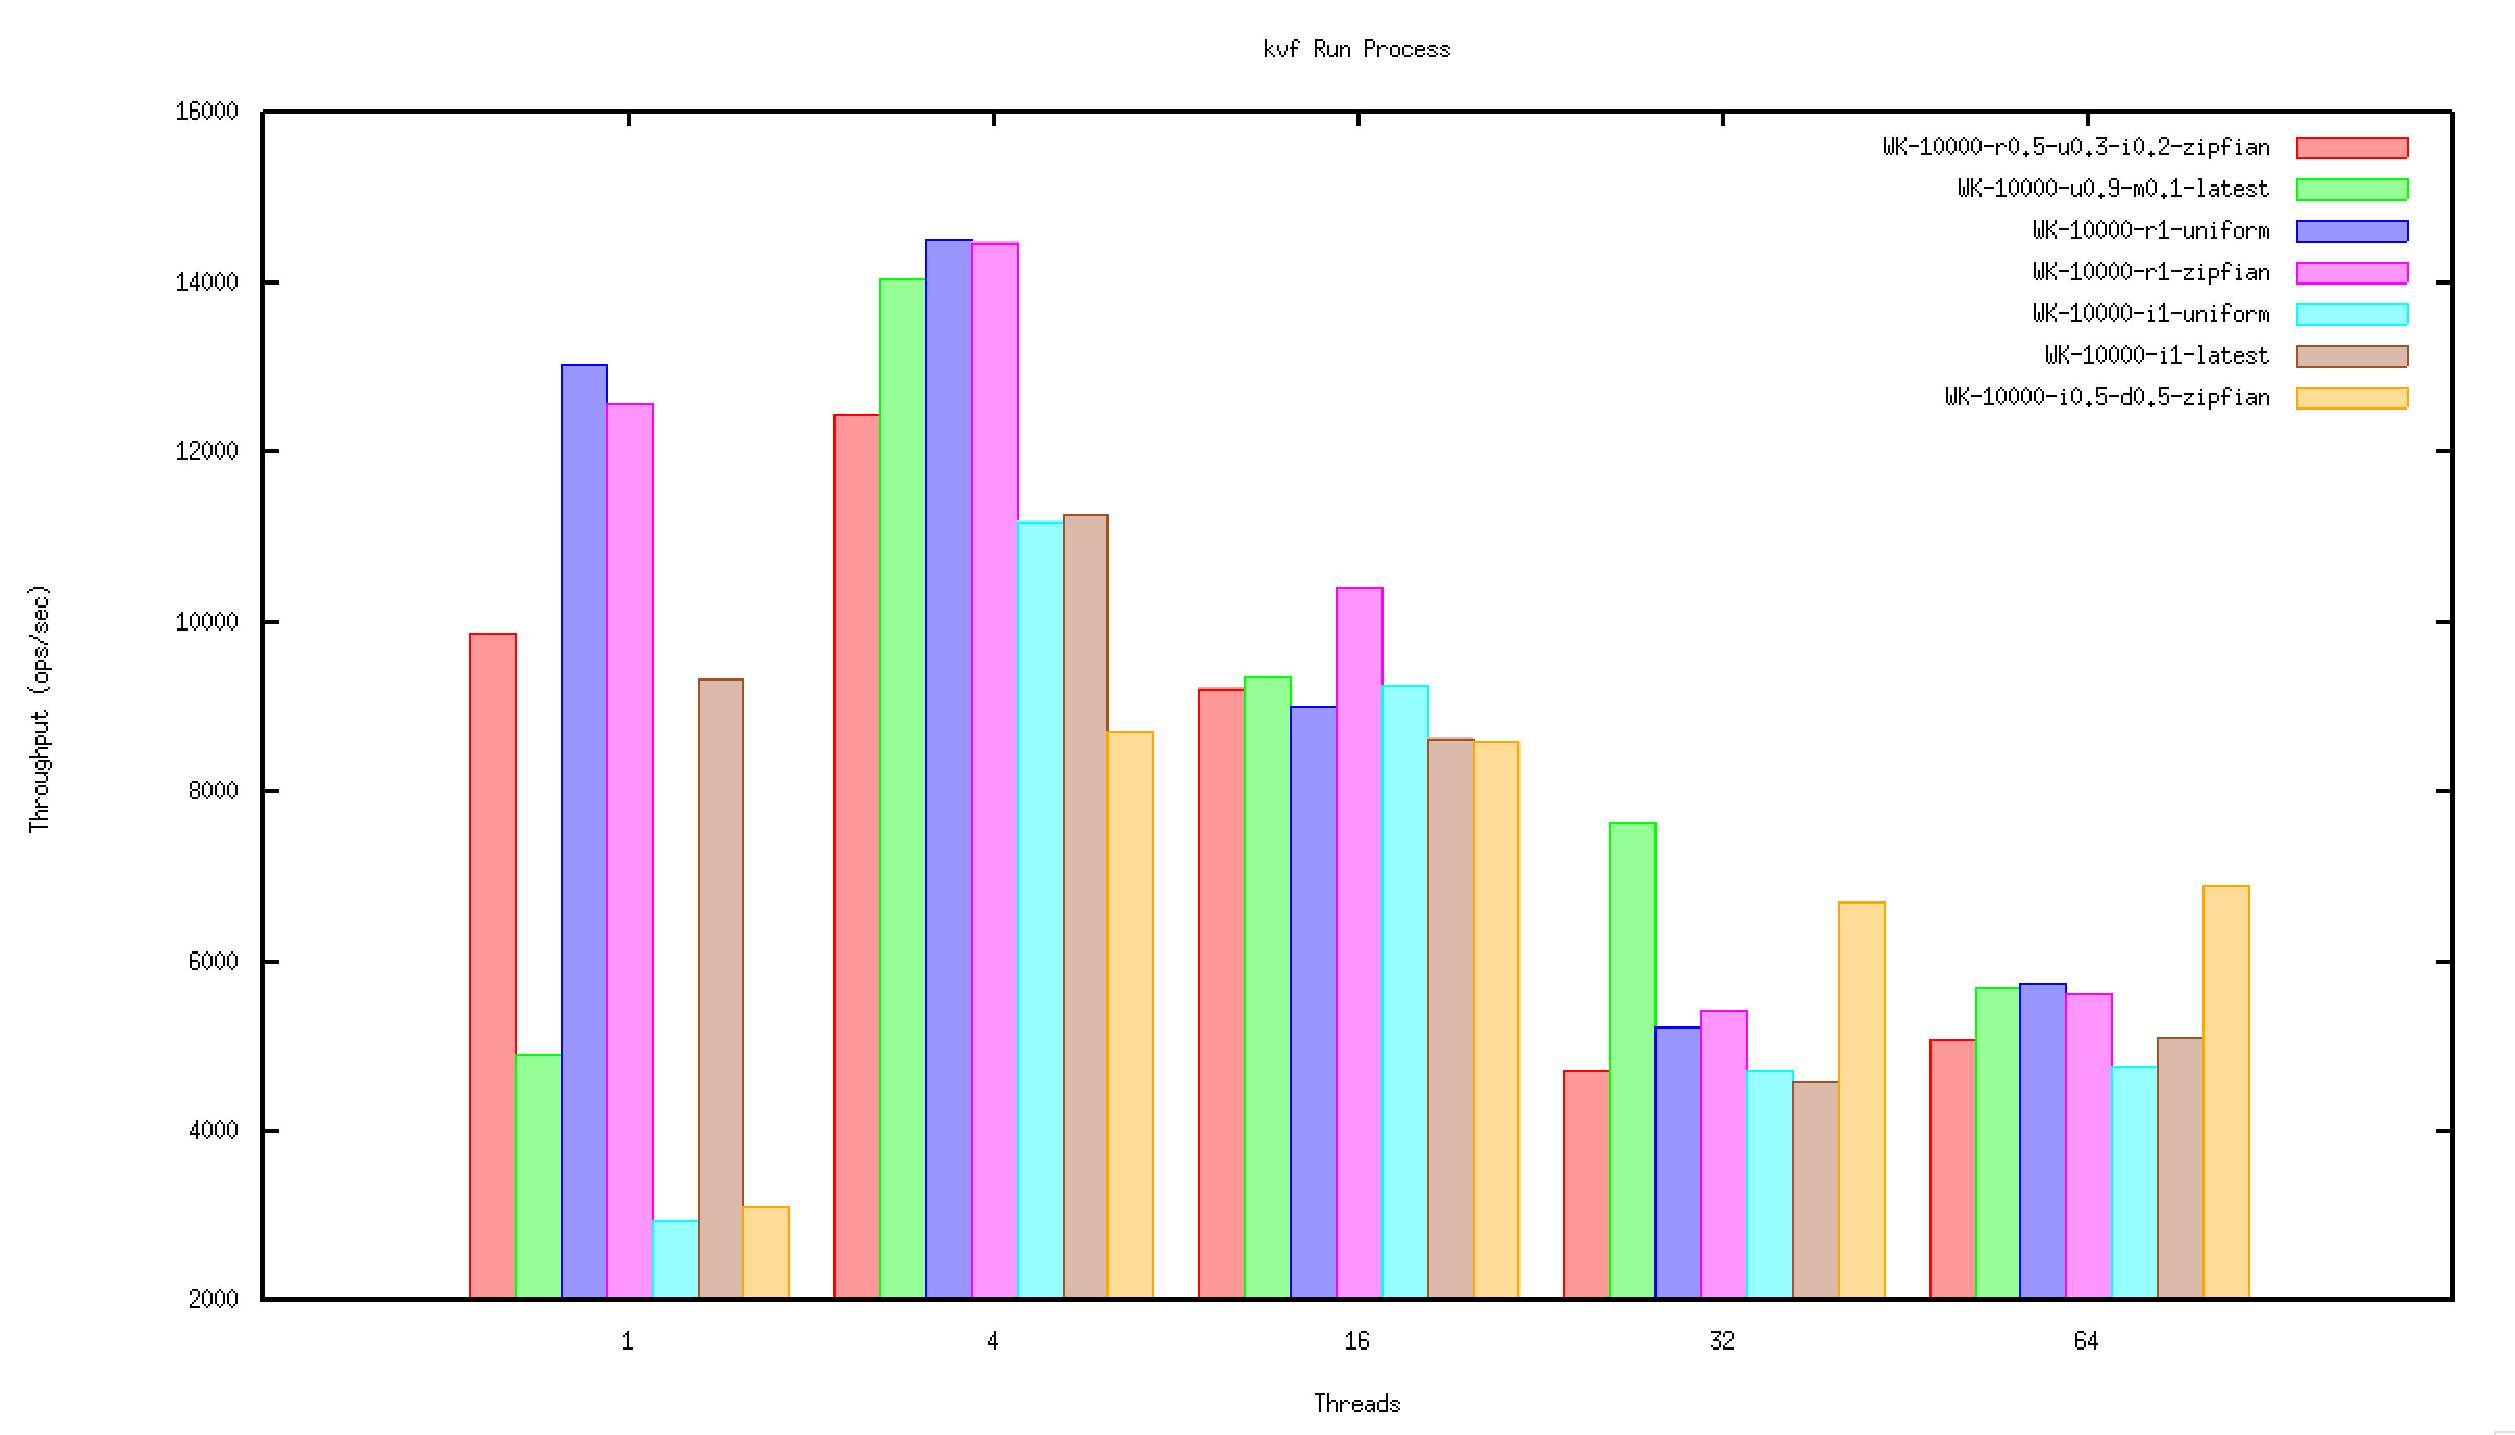
\includegraphics[width=13.9cm]{img/figure14.pdf}
\end{center}

	图中测试了六种不同的任务集分别在1、4、16、32、64线程中总体的吞吐量统计图。除了总体的数据,还可以短读显示插入、读、删除等每一种操作单独的统计数据。

\begin{center}
	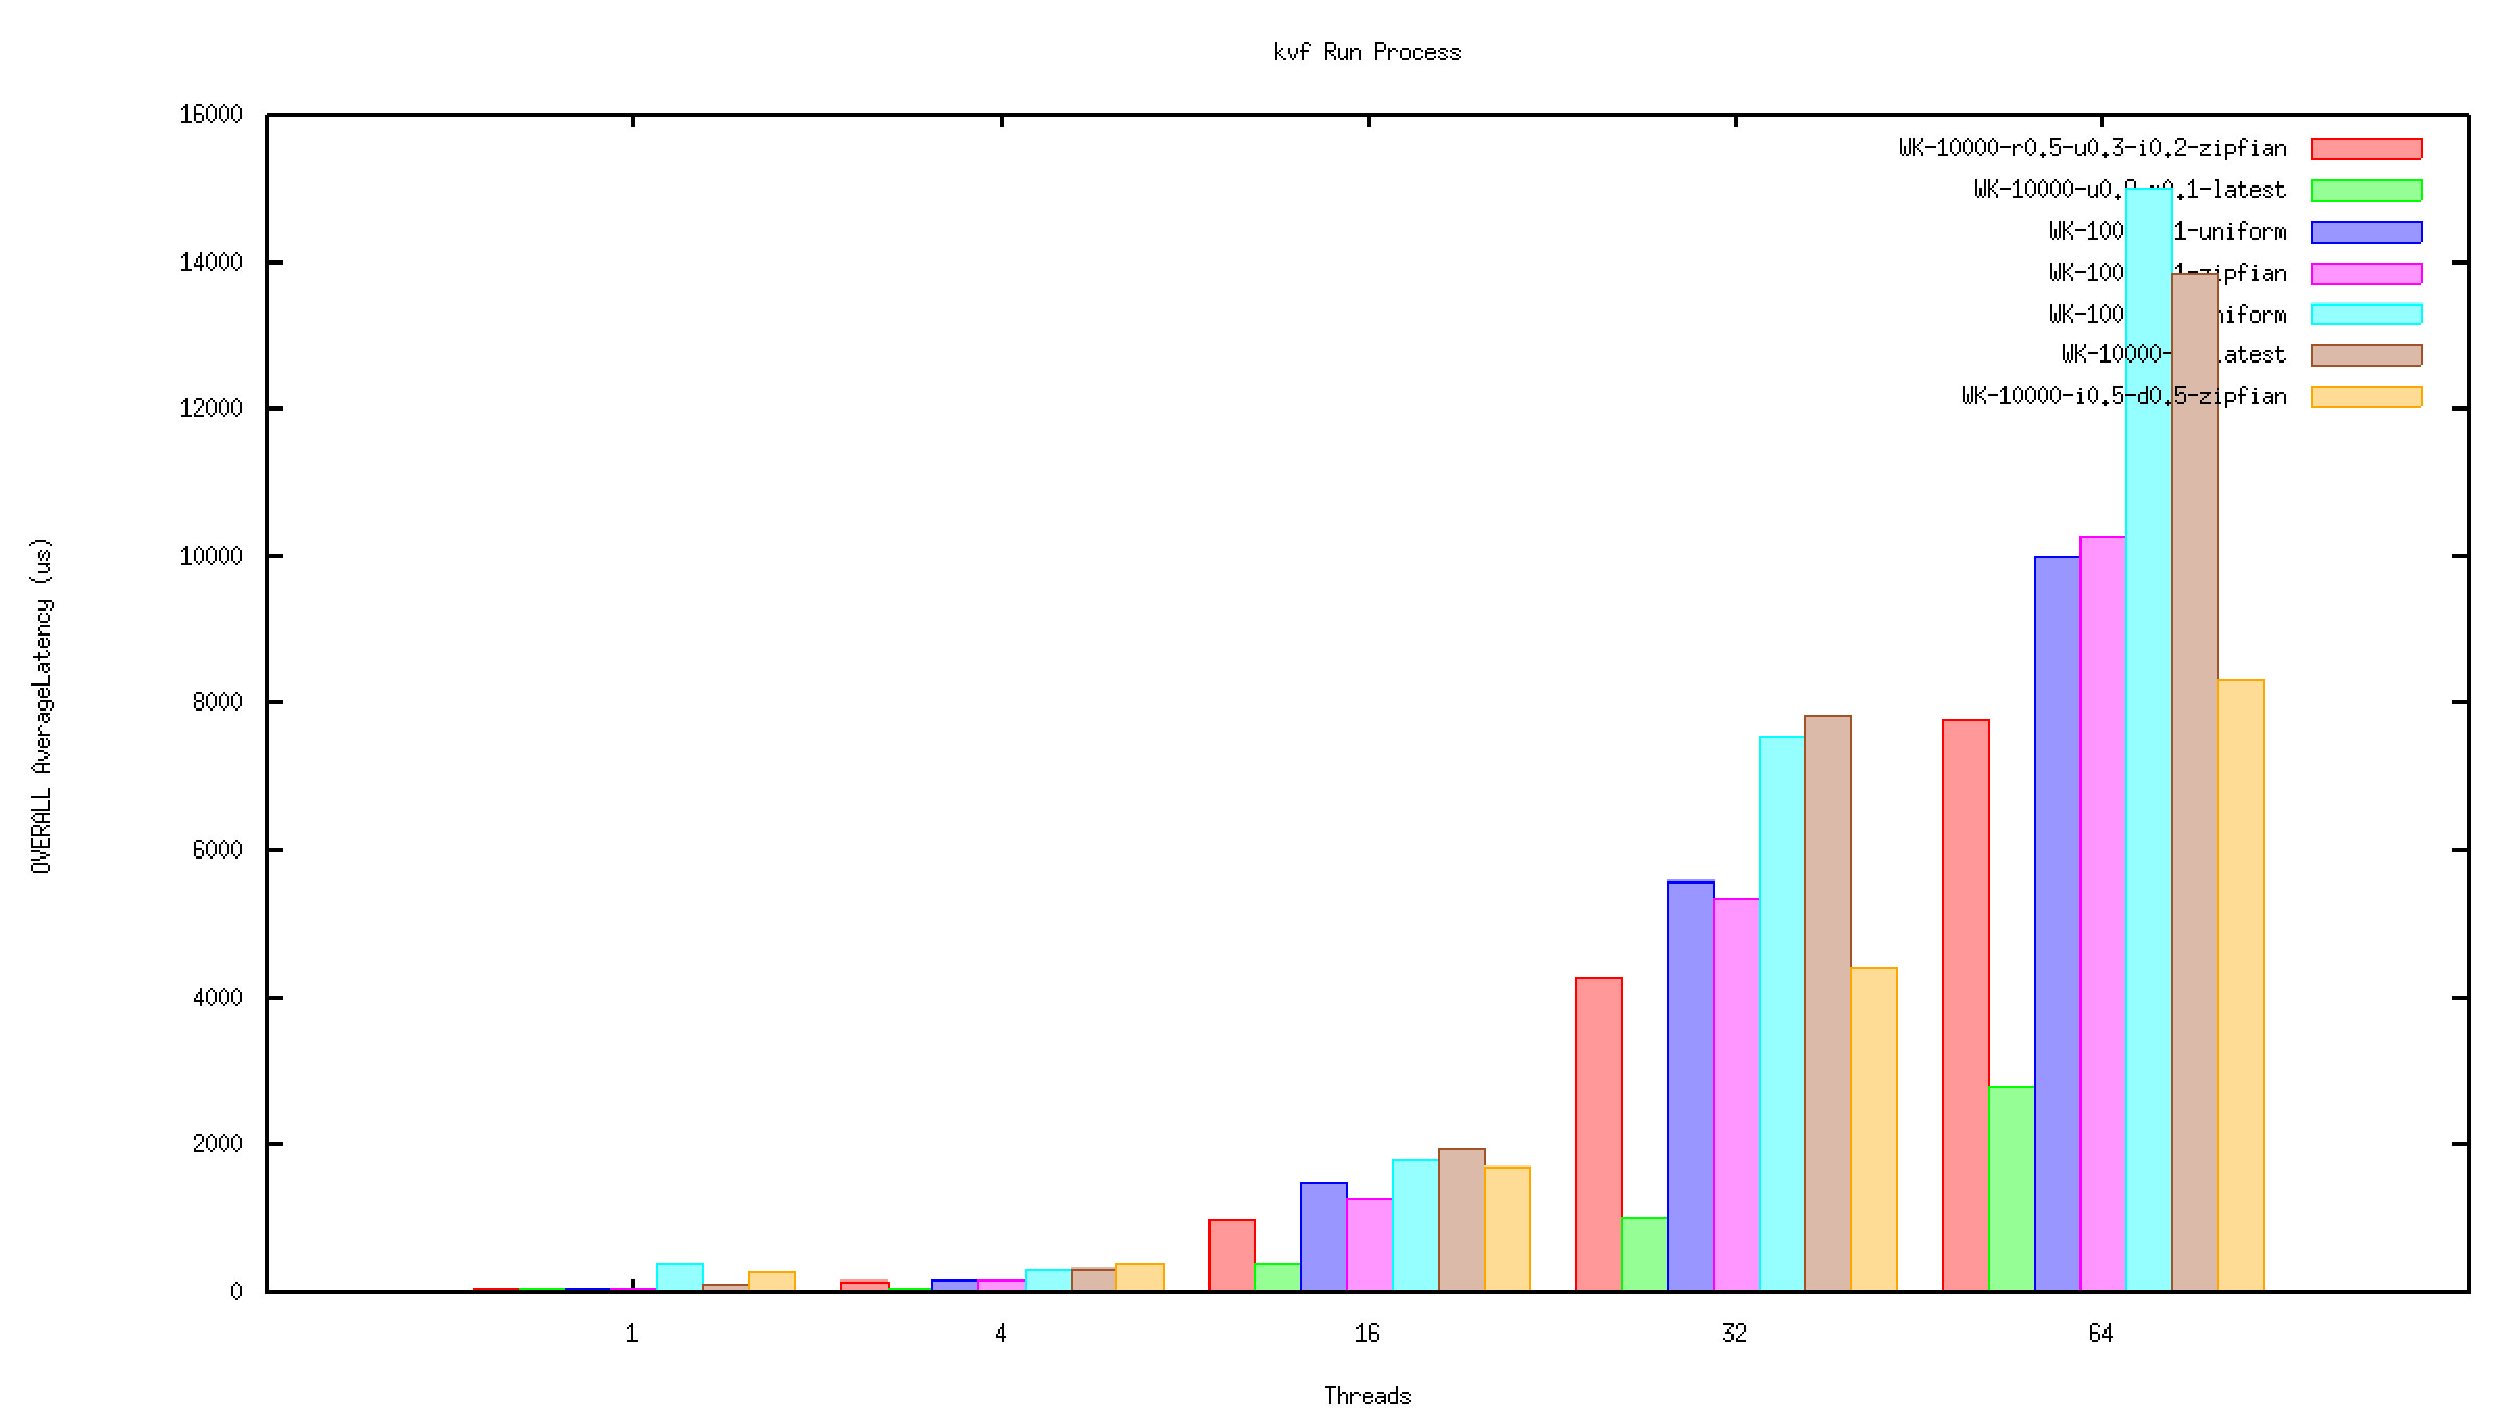
\includegraphics[width=13.9cm]{img/figure15.pdf}
\end{center}

	该图是同样测试的延迟统计。可以看出当线程数增加时延迟会越来越大。



%     - public int read(String table, String key, Set<String> 
%     - public int update(String table, String key, HashMap<String,
% public int update(String table, String key, HashMap<String,
%     - public void init() throws DBException {} 
%     - public int insert(String table, String key, HashMap<String,
	
%  public int read(String table, String key, Set<String> fields, 

% public int insert(String table, String key, HashMap<String,
% public int delete(String table, String key);
%     - public int delete(String table, String key);
% public int scan(String table, String startkey, int recordcount,

% java com.yahoo.ycsb.CommandLine -db com.yahoo.ycsb.db.MongoDbClient 

% 		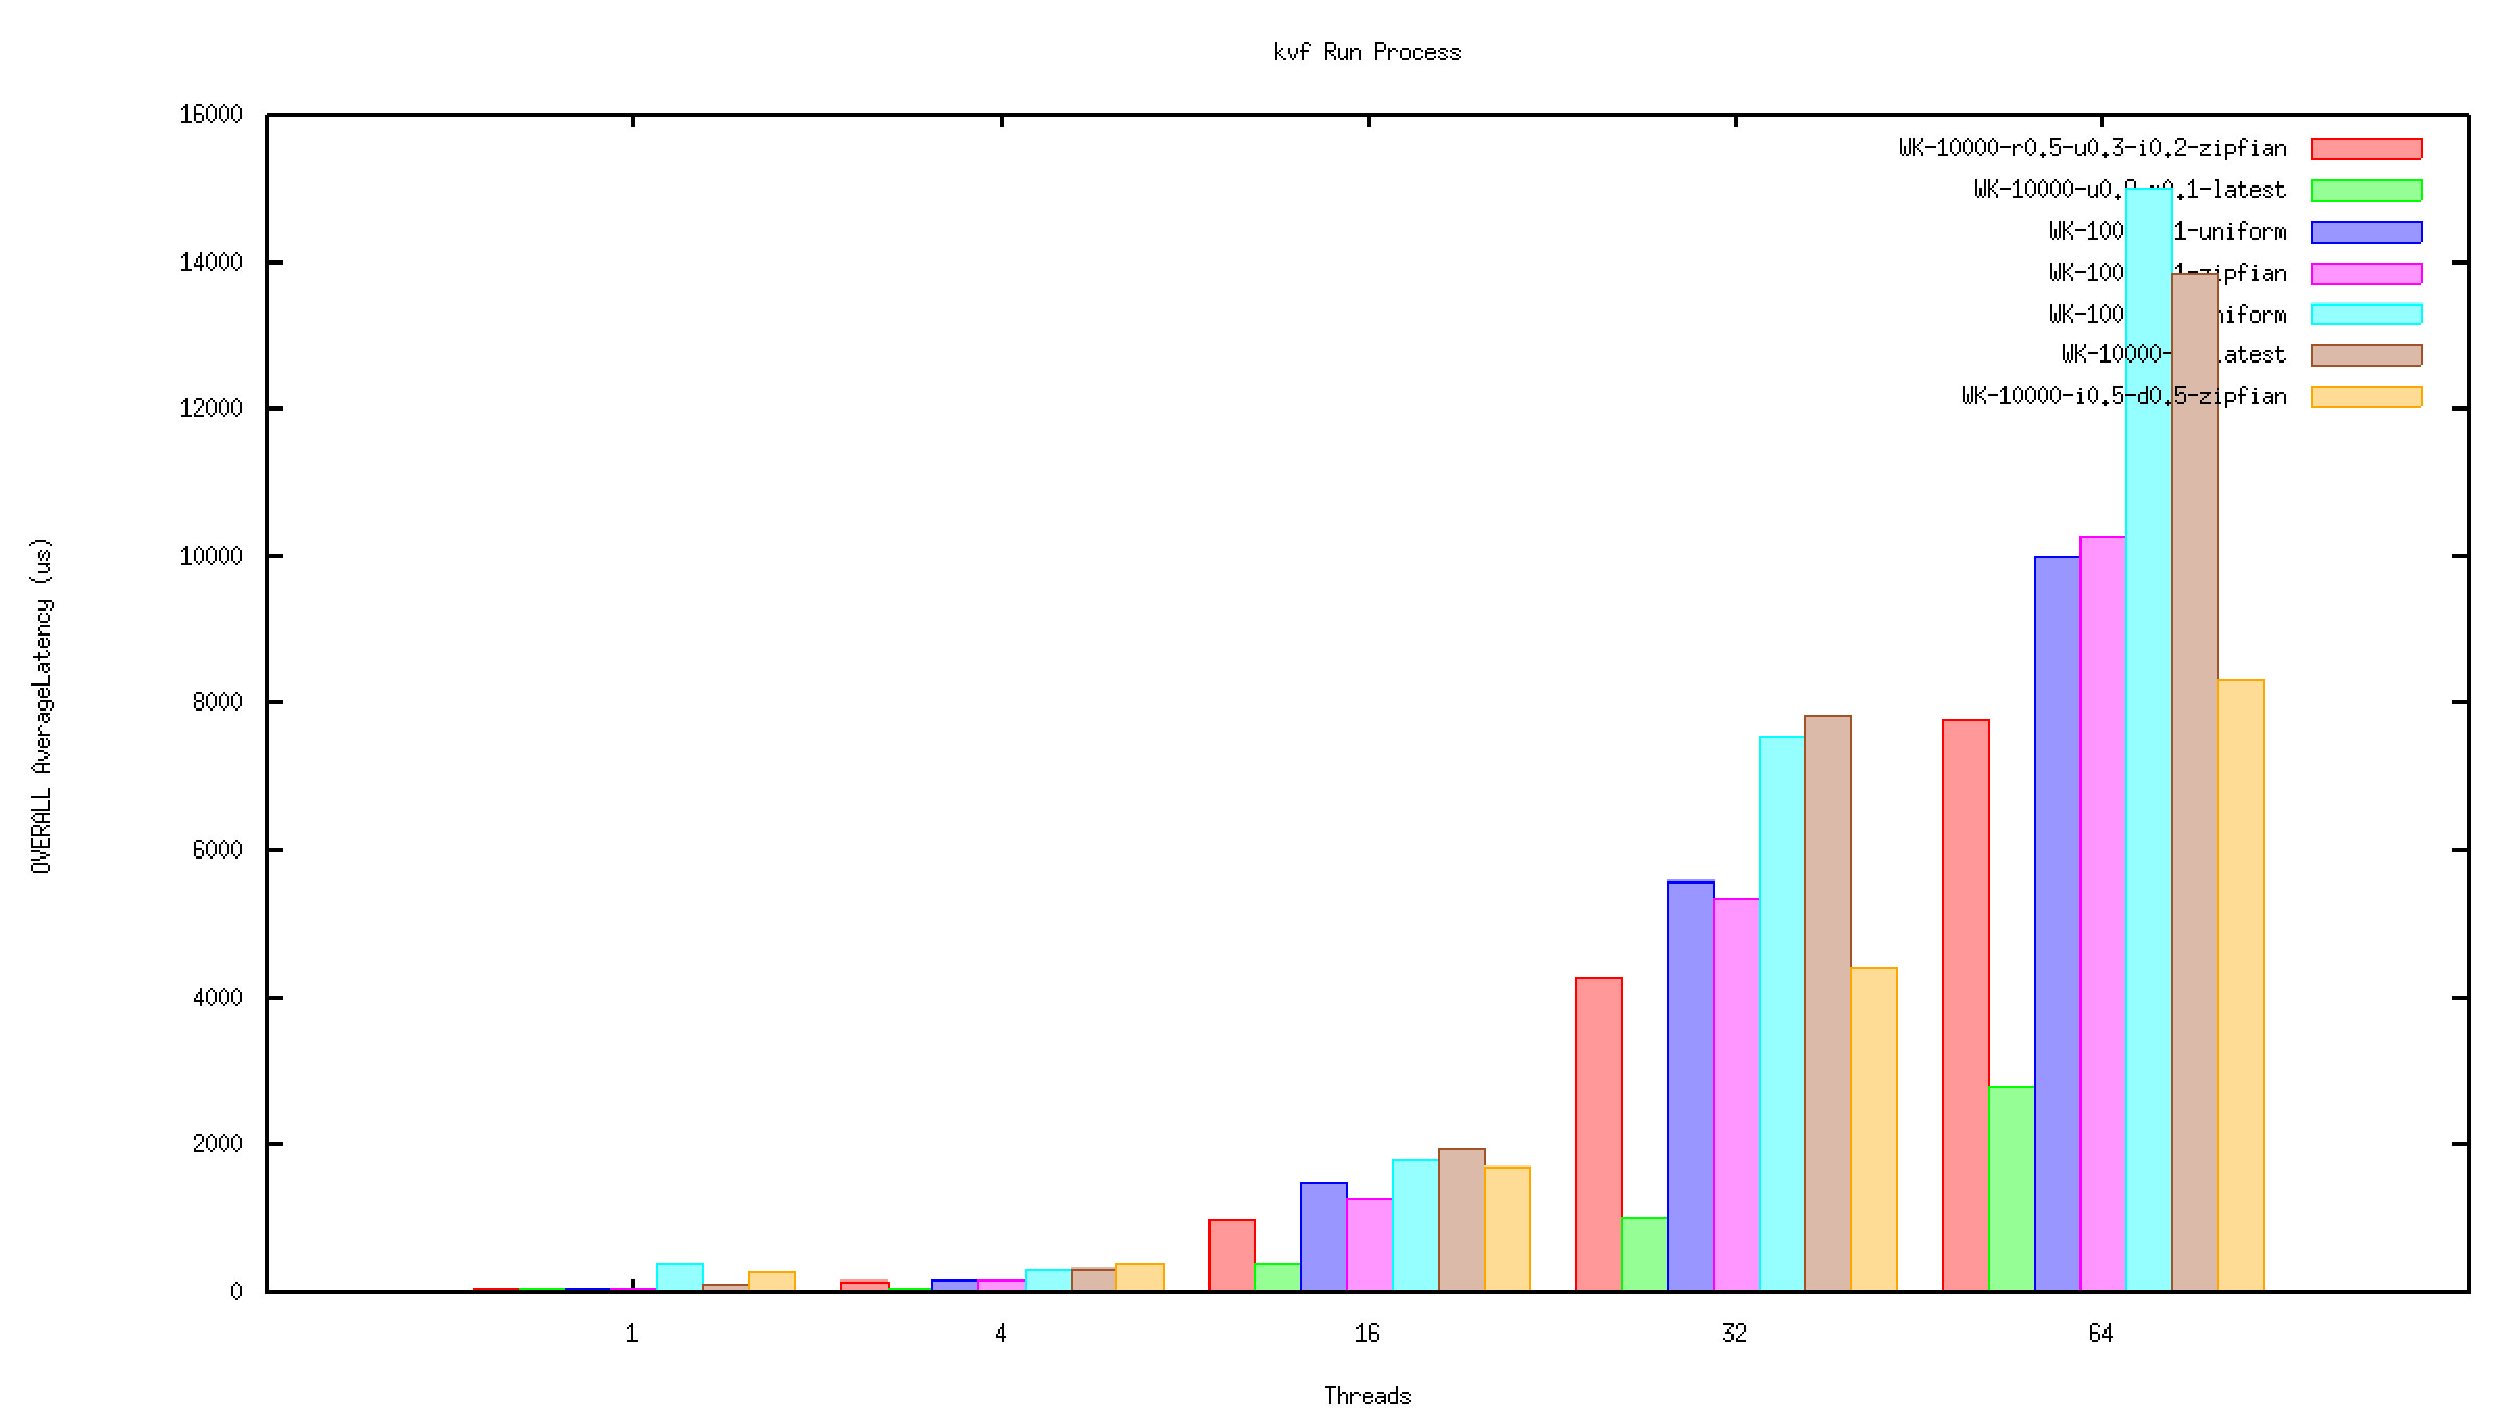
\includegraphics[width=15cm]{img/figure15.pdf}
% 	% 		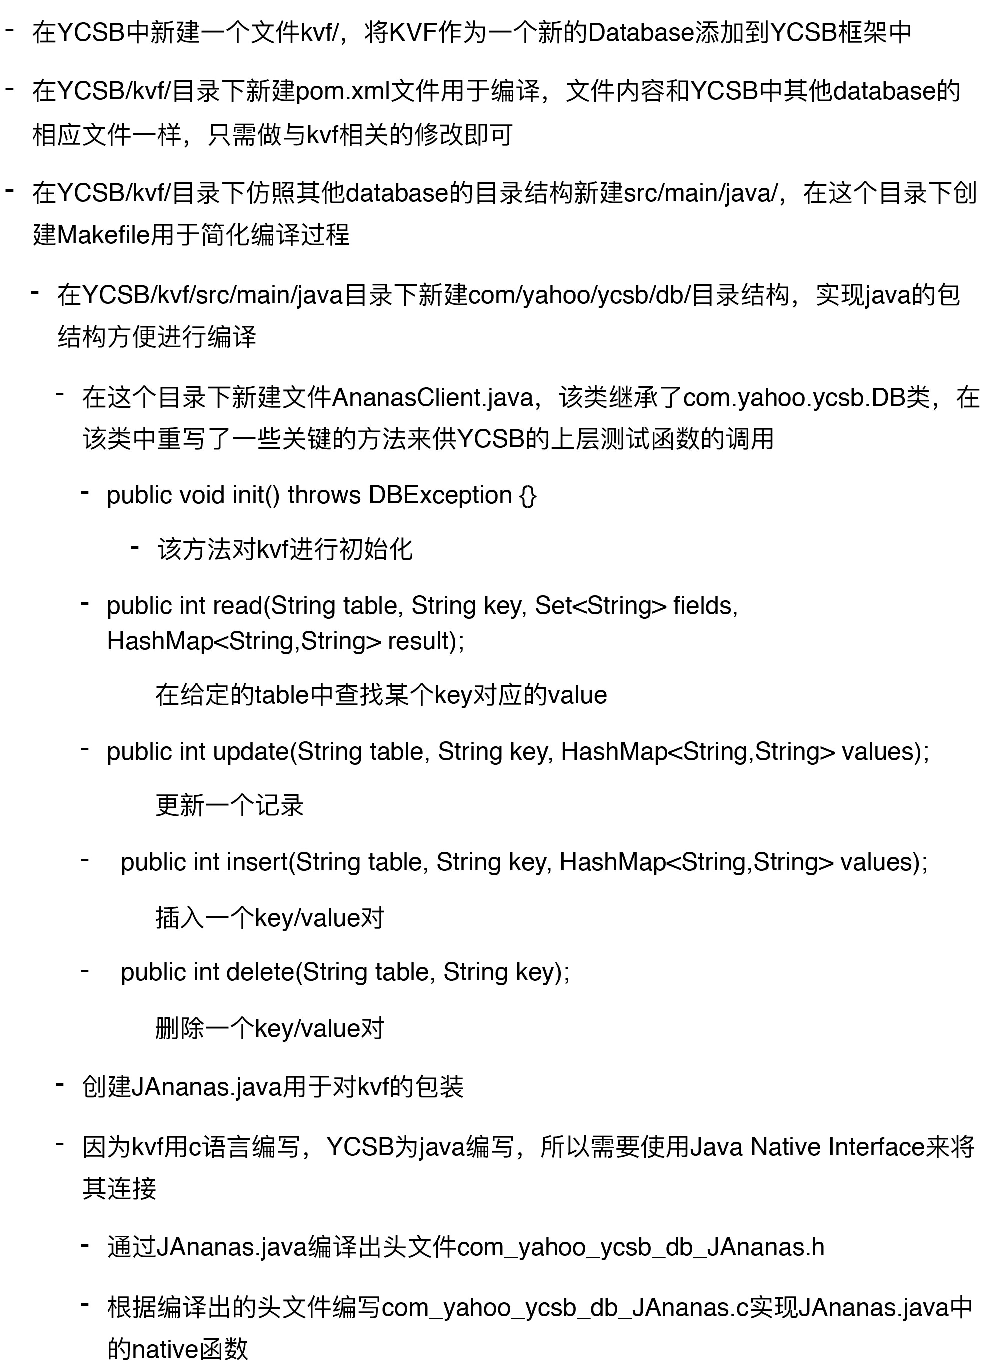
\includegraphics[width=13.9cm]{img/figure13.pdf}、
% 		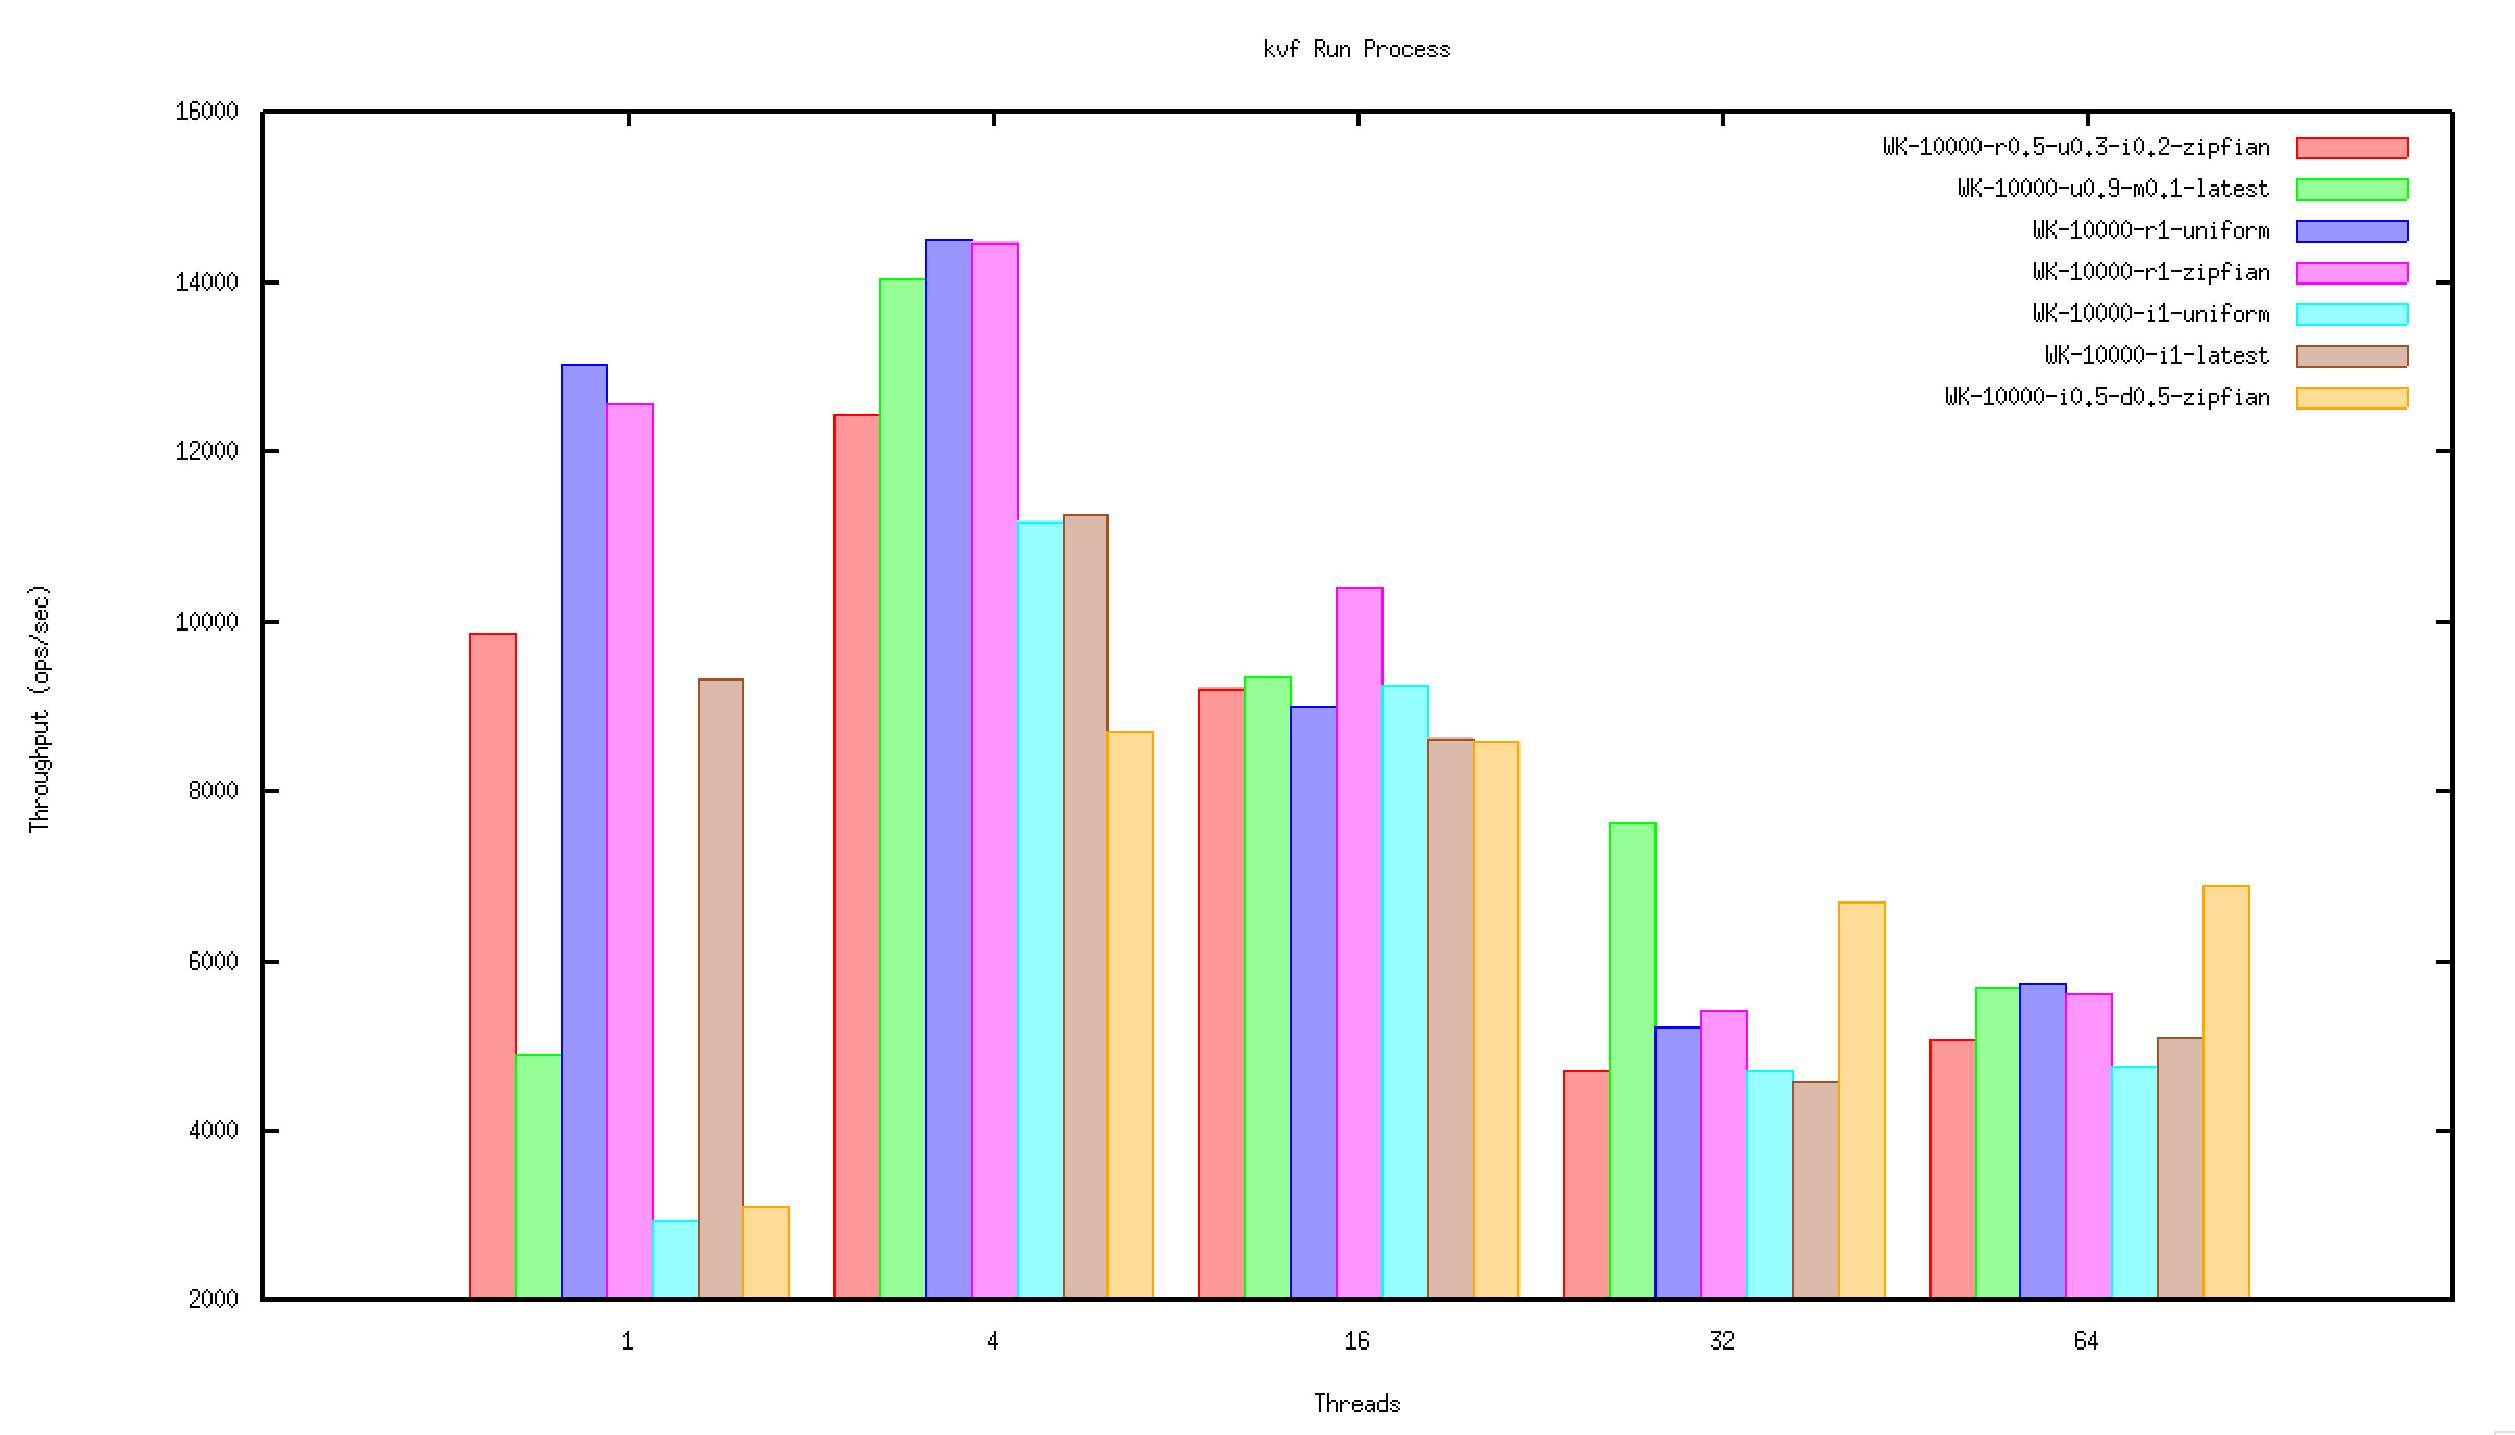
\includegraphics[width=15cm]{img/figure14.pdf}












%     [OVERALL], RunTime(ms), 309.0


	
%  	HashMap<String,String> result);

	

%     [UPDATE], AverageLatency(us), 1453.1361940298507


% 2 ms


	


% 	该方法对kvf进行初始化
%     String> values);
	
		


	


%     [UPDATE], 95thPercentileLatency(us), 2529.0
% 		\end{Verbatim}
% 191 ms
		
%     fields, HashMap<String,String> result);


%     operationcount=2000
	
% Type “help” for command line help

% Return code: 0




% //Insert a single record
% Return code: 1
		
%     [UPDATE], MaxLatency(us), 3625.0
%     [READ], Return=0, 1248

	
% //Update a single record
%     [INSERT], Operations, 216.0
%     [UPDATE], 99thPercentileLatency(us), 3119.0
	

%     [CLEANUP], 95thPercentileLatency(us), 1.0
%     [INSERT], AverageLatency(us), 2446.527777777778
% 	插入一个key/value对

% Connected.
% 	\end{center}



% 	删除一个key/value对





% 		\end{center}
% 		\end{Verbatim}
% 	\end{Verbatim}

%     [INSERT], Return=0, 216


% 	% 	\end{center}
%     [READ], MaxLatency(us), 7715.0
%     [OVERALL], Throughput(ops/sec), 6472.491909385113
%     [UPDATE], MinLatency(us), 208.0
%     readallfields=true
%     [INSERT], MaxLatency(us), 7903.0



% 	% \begin{center}



% 		\end{Verbatim}
%     requestdistribution=uniform
%     [INSERT], MinLatency(us), 643.0

  		
%     [READ], AverageLatency(us), 1267.5753205128206


% % vim:ts=4:sw=4


%     [UPDATE], Return=0, 536
		

	
% 	\begin{Verbatim}[frame = single]
		
		
	
%     [READ], 95thPercentileLatency(us), 2401.0
%     recordcount=1000
% 	\end{center}



% > insert brianfrankcooper first=brian last=cooper







% 	String> values);








% 	\end{Verbatim}
% \chapter{KVF测试系统YCSB}
%     updateproportion=0.25
	

% 		\end{Verbatim}



% //Delete a single record



% 		\end{Verbatim}
		
% 	Set<String> fields, Vector<HashMap<String,String>> result);

%     [READ], 99thPercentileLatency(us), 6383.0
%     readproportion=0.65

% 		\end{Verbatim}

%     workload=com.yahoo.ycsb.workloads.CoreWorkload
% 		\end{Verbatim}
% YCSB Command Line client

%     [CLEANUP], AverageLatency(us), 1.375


			
% 		\end{Verbatim}
% 		\begin{Verbatim}[frame = single]
% > quit
% 	String> values);
% 	\begin{center}
% 	更新一个记录

%     [CLEANUP], Operations, 16.0

%     [READ], MinLatency(us), 96.0
%   	String> values);
% 		\begin{Verbatim}[frame = single]
%     [CLEANUP], MinLatency(us), 0.0
  		
		
% 		\begin{Verbatim}[frame = single]

% 	\begin{Verbatim}[frame = none]
% 	\begin{Verbatim}[frame = none]
	
% 	\end{Verbatim}
		


% last=cooper
% % \pkuthssffaq % 中文测试文字。
% 	在给定的table中查找某个key对应的value



		
% first=brian
% 		\begin{Verbatim}[frame = single]

	
%     [READ], Operations, 1248.0
%     [INSERT], 95thPercentileLatency(us), 3661.0
% 		\begin{Verbatim}[frame = single]



% Start with “-help” for usage info
% 	\begin{Verbatim}[frame = none]
% 	\begin{center}
%     [INSERT], 99thPercentileLatency(us), 4455.0

% -p mongodb.url=mongodb://localhost:27017 -p mongodb.database=ycsb
	

%     [CLEANUP], MaxLatency(us), 9.0
% 		\end{Verbatim}
% //Perform a range scan
% 	\begin{Verbatim}[frame = single]


	

%     insertproportion=0.1
%     [UPDATE], Operations, 536.0
% \_id=brianfrankcooper

	
% 	\begin{Verbatim}[frame = none]
% 	\begin{Verbatim}[frame = single]
%     [CLEANUP], 99thPercentileLatency(us), 9.0
% 		\begin{center}


		
	
		
% > read brianfrankcooper



% 		\end{Verbatim}




% 		\begin{Verbatim}[frame = single]




%  //Read a single record
	% 结论。
	% Copyright (c) 2014,2016 Casper Ti. Vector
% Public domain.

\specialchap{结论}
% 中文测试文字。
	根据实际的使用情况,KV接口标准定义的API的语义概括了通用的KV模型,使上层应用可以使用一个统一的API接口来访问下层的KV存储。因此,KVF在实际的应用过程中有希望极大简化基于KV模型的应用的开发过程。另外KVF具有很好的扩展性,在上层应用开发的过程中可以灵活地根据自己的实际需要增加参数配置,定义自己的所需要的特定的数据结构,从而满足不同层次的需求。

	YCSB作为一个提供键值存储测试的平台,可以供很好的提测试方案,并且提供了易于使用的任务集配置方案,将其统计结果可视化处理之后我们可以很直观地对比不同任务集的各项数据,从而更好地进行分析。将YCSB和KVF进行连接是可行的,并且还可以直接与磁盘访问的底层函数相连接,从而可以分析和对比不同存储系统的性能损耗。


% vim:ts=4:sw=4


	% 正文中的附录部分。
	\appendix
	% 排版参考文献列表。bibintoc 选项使“参考文献”出现在目录中;
	% 如果同时要使参考文献列表参与章节编号,可将“bibintoc”改为“bibnumbered”。
	\printbibliography[heading = bibintoc]
	%\printbibliography[title = {Benchmarking Cloud Serving Systems with YCSB}, Brian F. Cooper, Adam Silberstein, Erwin Tam, Raghu Ramakrishnan, Russell Sears] %
	% 各附录。
	%% Copyright (c) 2014,2016 Casper Ti. Vector
% Public domain.

\chapter{附件}
%\pkuthssffaq % 中文测试文字。

% vim:ts=4:sw=4


	% 以下为正文之后的部分,默认不进行章节编号。
	\backmatter
	% 致谢。
	% Copyright (c) 2014,2016 Casper Ti. Vector
% Public domain.

\chapter{致谢}
 % 中文测试文字。
 	随着论文的结束,我的大学生涯也接近尾声,在这里我要感谢大学四年里帮助过我的各位老师、同学、师兄师姐们,正是你们的支持和帮助才使得我顺利度过了人生中国年最为重要的四年。

 	首先要非常感谢我的班主任谢冰老师,在我困惑迷茫的时候给我提出很好的建议,并在很多地方给我很大的帮助。

 	感谢孙广宇老师帮助我选择这样一个具有实际意义并且具有一定挑战性的毕业设计题目,如果不是这次毕业设计,我可能不会对键值存储数据库有这么深的了解,也不会对Linux系统有如此深入的探索。同样非常感谢在完成毕设过程中耐心指导我的王鹏师兄和王晓阳师兄,没有你们的帮助我也不会如此顺利地完成自己的题目。

 	感谢孙广宇和李文新老师在申请季给予的帮助和支持。

 	感谢大学各位朋友们的鼓励和帮助,特别是在羽协和山鹰社认识的各位好友,因为你们我的大学生活才如此精彩。

 	最后要感谢家人们默默的付出和关怀。
% vim:ts=4:sw=4

	% 原创性声明和使用授权说明。
	% Copyright (c) 2008-2009 solvethis
% Copyright (c) 2010-2016 Casper Ti. Vector
% All rights reserved.
%
% Redistribution and use in source and binary forms, with or without
% modification, are permitted provided that the following conditions are
% met:
%
% * Redistributions of source code must retain the above copyright notice,
%   this list of conditions and the following disclaimer.
% * Redistributions in binary form must reproduce the above copyright
%   notice, this list of conditions and the following disclaimer in the
%   documentation and/or other materials provided with the distribution.
% * Neither the name of Peking University nor the names of its contributors
%   may be used to endorse or promote products derived from this software
%   without specific prior written permission.
%
% THIS SOFTWARE IS PROVIDED BY THE COPYRIGHT HOLDERS AND CONTRIBUTORS "AS
% IS" AND ANY EXPRESS OR IMPLIED WARRANTIES, INCLUDING, BUT NOT LIMITED TO,
% THE IMPLIED WARRANTIES OF MERCHANTABILITY AND FITNESS FOR A PARTICULAR
% PURPOSE ARE DISCLAIMED. IN NO EVENT SHALL THE COPYRIGHT HOLDER OR
% CONTRIBUTORS BE LIABLE FOR ANY DIRECT, INDIRECT, INCIDENTAL, SPECIAL,
% EXEMPLARY, OR CONSEQUENTIAL DAMAGES (INCLUDING, BUT NOT LIMITED TO,
% PROCUREMENT OF SUBSTITUTE GOODS OR SERVICES; LOSS OF USE, DATA, OR
% PROFITS; OR BUSINESS INTERRUPTION) HOWEVER CAUSED AND ON ANY THEORY OF
% LIABILITY, WHETHER IN CONTRACT, STRICT LIABILITY, OR TORT (INCLUDING
% NEGLIGENCE OR OTHERWISE) ARISING IN ANY WAY OUT OF THE USE OF THIS
% SOFTWARE, EVEN IF ADVISED OF THE POSSIBILITY OF SUCH DAMAGE.

{
	\CTEXsetup[
		format+ = {\centering}, beforeskip = {40bp}, afterskip = {15bp}
	]{section}

	% 学校书面要求本页面不要页码,但在给出的 Word 模版中又有页码且编入了目录。
	% 此处以 Word 模版为实际标准进行设定。
	\specialchap{北京大学学位论文原创性声明和使用授权说明}
	\mbox{}\vspace*{-3em}
	\section*{原创性声明}

	本人郑重声明:
	所呈交的学位论文,是本人在导师的指导下,独立进行研究工作所取得的成果。
	除文中已经注明引用的内容外,
	本论文不含任何其他个人或集体已经发表或撰写过的作品或成果。
	对本文的研究做出重要贡献的个人和集体,均已在文中以明确方式标明。
	本声明的法律结果由本人承担。
	\vskip 1em
	\rightline{%
		论文作者签名:\hspace{5em}%
		日期:\hspace{2em}年\hspace{2em}月\hspace{2em}日%
	}

	\section*{%
		学位论文使用授权说明\\[-0.33em]
		\textmd{\zihao{5}(必须装订在提交学校图书馆的印刷本)}%
	}

	本人完全了解北京大学关于收集、保存、使用学位论文的规定,即:
	\begin{itemize}
		\item 按照学校要求提交学位论文的印刷本和电子版本;
		\item 学校有权保存学位论文的印刷本和电子版,
			并提供目录检索与阅览服务,在校园网上提供服务;
		\item 学校可以采用影印、缩印、数字化或其它复制手段保存论文;
		\item 因某种特殊原因需要延迟发布学位论文电子版,
			授权学校在 $\Box$\nobreakspace{}一年 /
			$\Box$\nobreakspace{}两年 /
			$\Box$\nobreakspace{}三年以后在校园网上全文发布。
	\end{itemize}
	\centerline{(保密论文在解密后遵守此规定)}
	\vskip 1em
	\rightline{%
		论文作者签名:\hspace{5em}导师签名:\hspace{5em}%
		日期:\hspace{2em}年\hspace{2em}月\hspace{2em}日%
	}

	% 若需排版二维码,请将二维码图片重命名为“barcode”,
	% 转为合适的图片格式,并放在当前目录下,然后去掉下面 2 行的注释。
	%\vfill\noindent
	%\includegraphics[height = 5em]{barcode}
}

% vim:ts=4:sw=4

\end{document}


% vim:ts=4:sw=4
